% This is samplepaper.tex, a sample chapter demonstrating the
% LLNCS macro package for Springer Computer Science proceedings;
% Version 2.20 of 2017/10/04
%
\documentclass[runningheads]{llncs}
%
% \usepackage{graphicx}
% \usepackage[dvipsnames]{xcolor}
%=====================================================
% NEWCOMMANDS
%=====================================================
\usepackage{lmodern}
\usepackage{mathtools}
\usepackage[utf8]{inputenc}
\usepackage{verbatim}
% \usepackage[english,french]{babel}
\usepackage[english]{babel}
\usepackage{latexsym}
\usepackage[normalem]{ulem}
\renewcommand{\ULdepth}{3pt}


\usepackage[outline]{contour}
\newcommand*{\fancy}[1]{{\color{white}\contour{black}{#1}}}


\usepackage{amsmath,amsthm,amsfonts,amssymb,empheq,relsize,alltt}
\usepackage{xparse}
%\usepackage{algorithm}
%\usepackage{algpseudocode}
\usepackage{algorithm2e}
\usepackage{bbdd}
\usepackage{bbm}
\DeclareMathAlphabet{\mathbbm}{U}{bbm}{m}{n}
% \usepackage{stmaryrd} CONFLICTING!!
\usepackage{subfig}
% \usepackage[singlelinecheck=0,font={sf,small},labelfont=bf]{caption, subfig}
% \captionsetup[subfigure]{subrefformat=simple,labelformat=simple,listofformat=subsimple,justification=raggedright}
\usepackage{cancel}
\usepackage{tikz}

\usepackage[noabbrev]{cleveref}
\let\chyperref\cref % Save the orginal command under a new name
\renewcommand{\cref}[1]{\hyperlink{#1}{\chyperref{#1}}} % Redefine the \cref command and explictely add the hyperlink. 
\usepackage{media9}
\usepackage{multimedia}
\usepackage{animate}
\usepackage[bbgreekl]{mathbbol}
%\usepackage{minted}

\newenvironment{questions}{\begin{list}{\arabic{nquestion}.}{\usecounter{nquestion}\setlength{\itemindent}{-0.5pt}\setlength{\listparindent}{250pt}}}{\unskip\end{list}}
%
\newcommand{\myparagraph}[1]{\subsubsection*{#1}}
% BEAMER
\newcommand{\ptl}[2]{{\large \textcolor{#2}{\textbf{#1}}}}
\newcommand{\pdfnewline}{\texorpdfstring{\newline}{ }} 
% Fill the vertical space in a slide (to put text at the bottom)
\newcommand{\framefill}{\vskip0pt plus 1filll}

\usepackage[skins,theorems]{tcolorbox}
\tcbset{highlight math style={enhanced,
  colframe=blue,boxrule=0.4pt,colback=white,arc=0pt,boxrule=0.2pt}}
\newcommand{\cit}[1]{{\tiny \textbf{#1}}}
% TEXTBLOCK
\newcommand{\txb}[4]{
\begin{textblock}{#1}(#2,#3)
	#4
\end{textblock}
}
\newcommand{\blk}[2]{
\begin{block}{#1}
	#2
\end{block}
}
\newcommand{\eblk}[2]{
\begin{exampleblock}{#1}
	#2
\end{exampleblock}
}
\newcommand{\ablk}[2]{
\begin{alertblock}{#1}
	#2
\end{alertblock}
}

\newcommand{\frm}[2]{
\begin{frame}{#1}
	#2
\end{frame}
}
\newcommand{\itmz}[1]{
\begin{itemize}
	#1
\end{itemize}
}
% INCLUDE GRAPHICS WIDTH
\newcommand{\igwf}[2]{
\includegraphics[keepaspectratio,width=#2]{#1}
}
% INCLUDE GRAPHICS HEIGHT
\newcommand{\ighf}[2]{
	\includegraphics[keepaspectratio,height=#2]{#1}
}
% SUBFIGURE
\newcommand{\subf}[2]{
\subfloat[#2]{#1\label{fig:#1}}
}
% SUBFIGURE WIDTH
\newcommand{\subfw}[3]{
	\subfloat[#3]{\igwf{#1}{#2}\label{fig:#1}}
}
% SUBFIGURE HEIGHT
\newcommand{\subfh}[3]{
	\subfloat[#3]{\ighf{#1}{#2}\label{fig:#1}}
}
% BEGIN FIGURE
\newcommand{\bfc}[3]{
\begin{figure}[ht!]
	\centering
	#1
	\caption{#2\label{fig:#3}}
\end{figure}
}
% BEGIN WRAPPED FIGURE
\usepackage{wrapfig}
\usepackage{capt-of}

\DeclareDocumentCommand{\bwfc}{ O{} O{} O{} O{l} O{20mm}}{
	\begin{wrapfigure}{#4}{#5}
		\begin{center}
			#1
			\captionof{figure}{#2}\label{fig:#3}
		\end{center}
\end{wrapfigure}
}

% EQUATION
\newcommand{\beq}[2]{
\begin{equation}
	#1
	\label{eq:#2}
\end{equation}
}
\DeclareDocumentCommand{\beqo}{ O{} O{} O{} }{
	\begin{equation}
	#1
	\label#3{eq:#2}
	\end{equation}
}
\DeclareDocumentCommand{\beqh}{ O{} O{} O{}  O{} }{
	\begin{equation}
	#1
	\hypertarget#3{#4}{\label#3{eq:#2}}
	\end{equation}
}


\DeclareDocumentCommand{\bsys}{ O{} O{} O{} }{
	\begin{empheq}[left=#1\empheqlbrace]{align}
	#2
	\label{eq:#3}
	\end{empheq}
}

\DeclareDocumentCommand{\bmat}{ O{} O{}  }{
	  \begin{bmatrix}
	  	\begin{array}{#2}
		#1
	\end{array}
	\end{bmatrix}
}
\DeclareDocumentCommand{\barr}{ O{} }{
	\begin{array}{c|c}
		#1
	\end{array}
}
%\usepackage{keyval}
%\makeatletter
%\define@key{janbertdims}{l}{\def\janbert@l{#1}}
%\define@key{janbertdims}{w}{\def\janbert@w{#1}}
%\define@key{janbertdims}{h}{\def\janbert@h{#1}}
%% initialize; change here to your preferred values
%\setkeys{janbertdims}{
%	l=1,        
%	w=1,    
%	h=1,
%}
%
%\newcommand\dimsEN[1][]{%
%	\begingroup
%	\setkeys{janbertdims}{#1}% the current values
%	The dimensions ($\mathrm{L} \times \mathrm{W} \times \mathrm{H}$)
%	of the room are
%	$\janbert@l \times \janbert@w \times \janbert@h$%
%	\endgroup
%}
%\makeatother
%
%	\dimsEN
%	
%	\dimsEN[h=3]
%	
%	\dimsEN[h=4,w=2]
%	
%	\dimsEN[w=3,l=5,h=2]
% GGD
\newcommand{\gggd}{$\frac{\text{G}}{\text{G}_\text{max}}-\gamma-\text{D}$ curves }
% KKNPP
\newcommand{\kka}[1][Nuclear Power Plant]{Kashiwazaki-Kariwa #1 }
% NCO
\newcommand{\NCO}{ \textit{Niigata-Ken Ch\={u}etsu-Oki} }
% TEPCO
\newcommand{\TEPCO}{ \textit{Tokyo Electric Power Company} }
% VS/VP/VS30
\newcommand{\vsth}{ V$_\text{S,30}$ }
\newcommand{\vs}{$V_{S}$ }
\newcommand{\vp}{$V_{P}$ }

\newcommand{\N}{\mathbb{N}}
\newcommand{\R}{\mathbb{R}}
\newcommand{\Z}{\mathbb{Z}}
%\newcommand{\C}{\mathbb{C}}
\DeclareDocumentCommand{\opercal}{O{}O{}O{}}{\ensuremath{\mathcal{#1}_{#2}^{#3}}}
\DeclareDocumentCommand{\operbb}{O{}O{}O{}}{\ensuremath{\mathbb{#1}_{#2}^{#3}}}
% VECTOR
\newcommand{\vct}[3]{\ensuremath{\boldsymbol{#1}_{#2}^{#3} }}
\DeclareDocumentCommand{\ebv}{ O{} O{} O{} }{\vct{e}{#1}{#2}#3}
\DeclareDocumentCommand{\debv}{ O{} O{} O{} }{\vct{\dot{e}}{#1}{#2}#3}
\DeclareDocumentCommand{\Phibv}{ O{} O{} O{} }{\vct{\Phi}{#1}{#2}#3}
\DeclareDocumentCommand{\ibv}{ O{} O{} O{} }{\vct{i}{#1}{#2}#3}

\DeclareDocumentCommand{\ione}{ O{} O{} }{\vct{i}{1}{#1}#2}
\DeclareDocumentCommand{\itwo}{ O{} O{} }{\vct{i}{2}{#1}#2}
\DeclareDocumentCommand{\ithree}{ O{} O{} }{\vct{i}{3}{#1}#2}
\DeclareDocumentCommand{\ivm}{ O{} O{} }{\vct{i}{m}{#1}#2}
\DeclareDocumentCommand{\ivn}{ O{} O{} }{\vct{i}{n}{#1}#2}
\DeclareDocumentCommand{\ivp}{ O{} O{} }{\vct{i}{p}{#1}#2}
\DeclareDocumentCommand{\ieta}{ O{} O{} }{\vct{i}{\eta}{#1}#2}
\DeclareDocumentCommand{\ix}{ O{} O{} }{\vct{i}{x}{#1}#2}
\DeclareDocumentCommand{\iy}{ O{} O{} }{\vct{i}{y}{#1}#2}

\DeclareDocumentCommand{\ir}{ O{} O{} O{} }{\vct{i}{r_{#1}}{#2}#3}
\DeclareDocumentCommand{\ith}{ O{} O{} O{} }{\vct{i}{\theta_{#1}}{#2}#3}
\DeclareDocumentCommand{\iz}{ O{} O{} O{} }{\vct{i}{z_{#1}}{#2}#3}
\DeclareDocumentCommand{\ixi}{ O{} }{\ibv[\xi]#1}
\DeclareDocumentCommand{\iXone}{ O{} }{\ibv[\chi_1]#1}
\DeclareDocumentCommand{\iXtwo}{ O{} }{\ibv[\chi_2]#1}
% beams
\DeclareDocumentCommand{\exi}{ O{} O{} }{\vct{e}{\xi}{#1}#2}
\DeclareDocumentCommand{\eXone}{ O{} }{\ebv[\chi_1]#1}
\DeclareDocumentCommand{\eXtwo}{ O{} }{\ebv[\chi_2]#1}
\DeclareDocumentCommand{\pG}{O{G}}{\pv[#1]}
\DeclareDocumentCommand{\pGp}{O{G} O{'}}{\pv[#1][#2]}
\DeclareDocumentCommand{\psigma}{O{\Sigma}}{\pv[#1]}
\DeclareDocumentCommand{\xG}{O{G}}{\xv[#1]}
\DeclareDocumentCommand{\xGo}{O{G_0}}{\xv[#1]}

\DeclareDocumentCommand{\xGp}{O{G} O{'}}{\xv[#1][#2]}
\DeclareDocumentCommand{\xGop}{O{G_0} O{'}}{\xv[#1][#2]}
\DeclareDocumentCommand{\xsigma}{O{\Sigma}}{\xv[#1]}
\DeclareDocumentCommand{\xsigmao}{O{\Sigma_0}}{\xv[#1]}
\DeclareDocumentCommand{\uG}{O{G}}{\uv[#1]}
\DeclareDocumentCommand{\uGo}{O{G_o}}{\uv[#1]}
\DeclareDocumentCommand{\uGp}{O{G}}{\uv[#1]}
\DeclareDocumentCommand{\uGop}{O{G_0} O{'}}{\uv[#1][#2]}
\DeclareDocumentCommand{\uGopp}{O{G_0} O{''}}{\uv[#1][#2]}
\DeclareDocumentCommand{\uGe}{O{Ge} O{}}{u_{#1}#2}
\DeclareDocumentCommand{\uGep}{O{Ge} O{'}}{u_{#1}^{#2}}
\DeclareDocumentCommand{\uGepp}{O{Ge} O{''}}{u_{#1}^{#2}}

\DeclareDocumentCommand{\uGoe}{O{G_0e} O{}}{u_{#1}#2}
\DeclareDocumentCommand{\uGoep}{O{G_0e} O{'}}{u_{#1}^{#2}}
\DeclareDocumentCommand{\uGoepp}{O{G_0e} O{''}}{u_{#1}^{#2}}

\DeclareDocumentCommand{\usigma}{O{\Sigma}}{\uv[#1]}
\DeclareDocumentCommand{\uGsigma}{O{G\Sigma}}{\uv[#1]}
\DeclareDocumentCommand{\uGsigmap}{O{G\Sigma} O{'}}{\uv[#1][#2]}
\DeclareDocumentCommand{\uGsigmapp}{O{G\Sigma} O{''}}{\uv[#1][#2]}


\DeclareDocumentCommand{\usigmao}{O{\Sigma_0}}{\uv[#1]}
\DeclareDocumentCommand{\uGosigma}{O{G_0\Sigma_0}}{\uv[#1]}
\DeclareDocumentCommand{\uGosigmap}{O{G_0\Sigma_0} O{'}}{\uv[#1][#2]}
\DeclareDocumentCommand{\uGosigmapp}{O{G_0\Sigma_0} O{''}}{\uv[#1][#2]}

\DeclareDocumentCommand{\uGperp}{O{G\vdash}}{\uv[#1]}
\DeclareDocumentCommand{\uGperpp}{O{G\vdash} O{'}}{\uv[#1][#2]}
\DeclareDocumentCommand{\uGperppp}{O{G\vdash} O{''}}{\uv[#1][#2]}

\DeclareDocumentCommand{\thetam}{ O{} O{} O{} }{\tens{\bbtheta}{#1}{\wedge}#3}
\DeclareDocumentCommand{\thetamp}{ O{} O{} O{} }{\tens{\bbtheta}{#1}{\wedge'}#3}
\DeclareDocumentCommand{\thetav}{ O{} O{} O{} }{\vct{\theta}{#1}{}#3}
\DeclareDocumentCommand{\thetavp}{ O{} O{} }{\vct{\theta}{#1}{'}#2}
\DeclareDocumentCommand{\thetavd}{ O{} O{} }{\vct{\dot{\theta}}{#1}{#2}}
\DeclareDocumentCommand{\thetavdd}{ O{} O{} }{\vct{\ddot{\theta}}{#1}{#2}}
\DeclareDocumentCommand{\Thetav}{ O{} O{} }{\vct{\Theta}{#1}{#2}}
\DeclareDocumentCommand{\Thetavd}{ O{} O{} }{\vct{\dot{\Theta}}{#1}{#2}}
\DeclareDocumentCommand{\Thetavdd}{ O{} O{} }{\vct{\ddot{\Theta}}{#1}{#2}}
\DeclareDocumentCommand{\thsigmap}{ O{} }{\vct{\theta}{\Sigma}{'}#1}
\DeclareDocumentCommand{\thsigmapp}{ O{} }{\vct{\theta}{\Sigma}{''}#1}
\DeclareDocumentCommand{\thsigma}{ O{\Sigma} O{} O{} }{\vct{\theta}{#1}{#2}#3}
\DeclareDocumentCommand{\thetae}{ O{e} O{} }{\theta_{#1}#2}
\DeclareDocumentCommand{\thetaep}{ O{e} O{'} }{\theta_{#1}^{#2}}
\DeclareDocumentCommand{\thetavperp}{ O{\vdash} O{} }{\vct{\theta}{\vdash}{#2}}
\DeclareDocumentCommand{\thetavzeroperp}{ O{\vdash} O{} }{\vct{\theta}{0\vdash}{#2}}



\DeclareDocumentCommand{\dduGv}{ O{} O{} O{} }{\vct{\ddot{u}}{G}{#2}#3}
\DeclareDocumentCommand{\dduGsigma}{ O{} O{} O{} }{\vct{\ddot{u}}{G\Sigma}{#2}#3}
\DeclareDocumentCommand{\ddthetav}{ O{} O{} O{} }{\vct{\ddot{\theta}}{#1}{#2}#3}
\DeclareDocumentCommand{\ddthetae}{}{\ensuremath{\ddot{\theta}_e}}
\DeclareDocumentCommand{\pthp}{ O{} }{\ensuremath{\pdp{\theta_{#1}}} }
\DeclareDocumentCommand{\stressref}{O{0}}{\ensuremath{\stress \phantom{}_{\text{#1}}}}

\DeclareDocumentCommand{\hv}{ O{} O{} O{} }{\vct{h}{#1}{#2}#3}
\DeclareDocumentCommand{\ov}{ O{} O{} O{} }{\vct{o}{#1}{#2}#3}
\DeclareDocumentCommand{\yv}{ O{} O{} O{} }{\vct{y}{#1}{#2}#3}
\DeclareDocumentCommand{\ytv}{ O{} O{} O{} }{\vct{\tilde{y}}{#1}{#2}#3}
\DeclareDocumentCommand{\dyv}{ O{} O{} O{} }{\vct{\dot{y}}{#1}{#2}#3}
\DeclareDocumentCommand{\ddyv}{ O{} O{} O{} }{\vct{\ddot{y}}{#1}{#2}#3}
\DeclareDocumentCommand{\pv}{ O{} O{} O{} }{\vct{p}{#1}{#2}#3}
\DeclareDocumentCommand{\dpv}{ O{} O{} O{} }{\vct{dp}{#1}{#2}#3}
\DeclareDocumentCommand{\Xv}{ O{} O{} O{} }{\vct{X}{#1}{#2}#3}
\DeclareDocumentCommand{\Xhv}{ O{} O{} O{} }{\vct{\hat X}{#1}{#2}#3}
\DeclareDocumentCommand{\Zhv}{ O{} O{} O{} }{\vct{\hat Z}{#1}{#2}#3}
\DeclareDocumentCommand{\xv}{ O{} O{} O{} }{\vct{x}{#1}{#2}#3}
\DeclareDocumentCommand{\xhv}{ O{} O{} O{} }{\vct{\hat x}{#1}{#2}#3}
\DeclareDocumentCommand{\zhv}{ O{} O{} O{} }{\vct{\hat z}{#1}{#2}#3}
\DeclareDocumentCommand{\dxv}{ O{} O{} O{} }{\vct{dx}{#1}{#2}#3}
\DeclareDocumentCommand{\Xtv}{ O{} O{} O{} }{\vct{\tilde{X}}{#1}{#2}#3}
\DeclareDocumentCommand{\Xt}{ O{} O{} O{} }{\tens{\mathbb{X}}{#1}{#2}#3}
\DeclareDocumentCommand{\xgv}{ O{} O{} O{} }{\vct{x}{g}{#1}#2}
\DeclareDocumentCommand{\ddxgv}{ O{} O{} O{} }{\vct{\ddot{x}}{g}{#1}#2}
\DeclareDocumentCommand{\tv}{ O{} O{} O{} }{\vct{t}{#1}{#2}#3}
\DeclareDocumentCommand{\fv}{ O{} O{} O{} }{\vct{f}{#1}{#2}#3}
\DeclareDocumentCommand{\fvi}{ O{} O{} O{} }{\vct{f}{#1}{-1}#3}
\DeclareDocumentCommand{\ftv}{ O{} O{} O{} }{\vct{\tilde{f}}{#1}{#2}#3}
\DeclareDocumentCommand{\Ft}{ O{} O{} O{} }{\tens{\mathbb{F}}{#1}{#2}#3}
\DeclareDocumentCommand{\kv}{ O{} O{} O{} }{\vct{k}{#1}{#2}#3}
\DeclareDocumentCommand{\khv}{ O{} O{} O{} }{\vct{\hat{k}}{#1}{#2}#3}
\DeclareDocumentCommand{\sv}{ O{} O{} O{} }{\vct{s}{#1}{#2}#3}
\DeclareDocumentCommand{\cv}{ O{} O{} O{} }{\vct{c}{#1}{#2}#3}
\DeclareDocumentCommand{\Cv}{ O{} O{} O{} }{\vct{C}{#1}{#2}#3}
\DeclareDocumentCommand{\Sv}{ O{} O{} O{} }{\vct{S}{#1}{#2}#3}
\DeclareDocumentCommand{\Nv}{ O{} O{} O{} }{\vct{N}{#1}{#2}#3}
\DeclareDocumentCommand{\muv}{ O{} O{} O{} }{\vct{\mu}{#1}{#2}#3}
\DeclareDocumentCommand{\dcv}{ O{} O{} O{} }{\vct{\dot{c}}{#1}{#2}#3}
\DeclareDocumentCommand{\ddcv}{ O{} O{} O{} }{\vct{\ddot{c}}{#1}{#2}#3}
\DeclareDocumentCommand{\ctv}{ O{} O{} O{} }{\vct{\tilde{c}}{#1}{#2}#3}
\DeclareDocumentCommand{\cbv}{ O{} O{} O{} }{\vct{\bar{c}}{#1}{#2}#3}
\DeclareDocumentCommand{\btv}{ O{} O{} O{} }{\vct{\tilde{b}}{#1}{#2}#3}
\DeclareDocumentCommand{\btt}{ O{} O{} O{} }{\tens{\tilde{\mathbbm{b}}}{#1}{#2}#3}
\DeclareDocumentCommand{\bbv}{ O{} O{} O{} }{\vct{\bar{b}}{#1}{#2}#3}
\DeclareDocumentCommand{\bbt}{ O{} O{} O{} }{\tens{\bar{\mathbbm{b}}}{#1}{#2}#3}
\DeclareDocumentCommand{\Ct}{ O{} O{} O{} }{\tens{\mathbb{C}}{#1}{#2}#3}
\DeclareDocumentCommand{\dv}{ O{} O{} O{} }{\vct{d}{#1}{#2}#3}
\DeclareDocumentCommand{\Dt}{ O{} O{} O{} }{\tens{\mathbb{D}}{#1}{#2}#3}
\DeclareDocumentCommand{\vV}{ O{} O{} O{} }{\vct{v}{#1}{#2}#3}
\DeclareDocumentCommand{\Vt}{ O{} O{} O{} }{\tens{\mathbb{V}}{#1}{#2}#3}
\DeclareDocumentCommand{\dvV}{ O{} O{} O{} }{\vct{dv}{#1}{#2}#3}
\DeclareDocumentCommand{\vt}{ O{} O{} O{} }{\tens{\mathbbm{v}}{#1}{#2}#3}
\DeclareDocumentCommand{\bv}{ O{} O{} O{} }{\vct{b}{#1}{#2}#3}
\DeclareDocumentCommand{\bt}{ O{} O{} O{} }{\tens{\mathbbm{b}}{#1}{#2}#3}
\DeclareDocumentCommand{\Bt}{ O{} O{} O{} }{\tens{\mathbb{B}}{#1}{#2}#3}
\DeclareDocumentCommand{\St}{ O{} O{} O{} }{\tens{\mathbb{S}}{#1}{#2}#3}

\DeclareDocumentCommand{\Vv}{ O{} O{} O{} }{\vct{V}{#1}{#2}#3}
\DeclareDocumentCommand{\qv}{ O{} O{} O{} }{\vct{q}{#1}{#2}#3}
\DeclareDocumentCommand{\Qt}{ O{} O{} O{} }{\tens{\mathbb{Q}}{#1}{#2}#3}
\DeclareDocumentCommand{\qvF}{ O{} O{} O{} }{\vct{\hat{q}}{#1}{#2}#3}
\DeclareDocumentCommand{\ddqv}{ O{} O{} O{} }{\vct{\ddot{q}}{#1}{#2}#3}
\DeclareDocumentCommand{\dqv}{ O{} O{} O{} }{\vct{\dot{q}}{#1}{#2}#3}
\DeclareDocumentCommand{\deltaqv}{ O{} O{} O{} }{\vct{\delta q}{#1}{#2}#3}
\DeclareDocumentCommand{\av}{ O{} O{} O{} }{\vct{a}{#1}{#2}#3}
\DeclareDocumentCommand{\avf}{ O{} O{} O{} }{\vct{\tilde{a}}{#1}{#2}#3}
\DeclareDocumentCommand{\at}{ O{} O{} O{} }{\tens{\mathbbm{a}}{#1}{#2}#3}
\DeclareDocumentCommand{\Tt}{ O{} O{} O{} }{\tens{\mathbb{T}}{#1}{#2}#3}
\DeclareDocumentCommand{\Gt}{ O{} O{} O{} }{\tens{\mathbb{G}}{#1}{#2}#3}

\DeclareDocumentCommand{\Sigmat}{ O{} O{} O{} }{\tens{\dSigma}{#1}{#2}#3}
\DeclareDocumentCommand{\At}{ O{} O{} O{} }{\tens{\mathbb{A}}{#1}{#2}#3}
\DeclareDocumentCommand{\Adt}{ O{} O{} O{} }{\tens{\dot{A}}{#1}{#2}#3}
\DeclareDocumentCommand{\Av}{ O{} O{} O{} }{\vct{A}{#1}{#2}#3}
\DeclareDocumentCommand{\tAv}{ O{} O{} O{} }{\vct{\tilde A}{#1}{#2}#3}
\DeclareDocumentCommand{\wv}{ O{} O{} O{} }{\vct{w}{#1}{#2}#3}
\DeclareDocumentCommand{\dwv}{ O{} O{} O{} }{\vct{\dot{w}}{#1}{#2}#3}
\DeclareDocumentCommand{\zv}{ O{} O{} O{} }{\vct{z}{#1}{#2}#3}
\DeclareDocumentCommand{\Zv}{ O{} O{} O{} }{\vct{Z}{#1}{#2}#3}
\DeclareDocumentCommand{\fm}{ O{} O{} O{} }{\vct{f}{#1}{#2}#3}
\DeclareDocumentCommand{\nv}{ O{} O{} O{} }{\vct{n}{#1}{#2}#3}
\DeclareDocumentCommand{\Nv}{ O{} O{} O{} }{\vct{N}{#1}{#2}#3}
\DeclareDocumentCommand{\Bv}{ O{} O{} O{} }{\vct{B}{#1}{#2}#3}
\DeclareDocumentCommand{\mv}{ O{} O{} O{} }{\vct{m}{#1}{#2}#3}
\DeclareDocumentCommand{\qv}{ O{} O{} O{} }{\vct{q}{#1}{#2}#3}
\DeclareDocumentCommand{\gv}{ O{} O{} O{} }{\vct{g}{#1}{#2}#3}
\DeclareDocumentCommand{\tauv}{ O{} O{} O{} }{\vct{\tau}{#1}{#2}#3}
\DeclareDocumentCommand{\tauvsigma}{ O{} O{} O{} }{\vct{\tau}{\Sigma}{#2}#3}
\DeclareDocumentCommand{\Nv}{ O{} O{} O{} }{\vct{N}{#1}{#2}#3}
\DeclareDocumentCommand{\Nm}{ O{} O{} O{} }{\tens{N}{#1}{#2}#3}
\DeclareDocumentCommand{\Rv}{ O{} O{} O{} }{\vct{R}{#1}{#2}#3}
\DeclareDocumentCommand{\Rm}{ O{} O{} O{} }{\tens{R}{#1}{#2}#3}
\DeclareDocumentCommand{\Rt}{ O{} O{} O{} }{\tens{\mathbb{R}}{#1}{#2}#3}
\DeclareDocumentCommand{\dRt}{ O{} O{} O{} }{\tens{\dot{\mathbb{R}}}{#1}{#2}#3}
\DeclareDocumentCommand{\Omegat}{ O{} O{} O{} }{\tens{\dOmega}{#1}{#2}#3}
\DeclareDocumentCommand{\OmegatT}{ O{} O{} O{} }{\tens{\dOmega}{#1}{T#2}#3}
\DeclareDocumentCommand{\omegav}{ O{} O{} O{} }{\vct{\omega}{#1}{#2}#3}
\DeclareDocumentCommand{\dOmegat}{ O{} O{} O{} }{\tens{\dot{\dOmega}}{#1}{#2}#3}

\DeclareDocumentCommand{\Mv}{ O{} O{} O{} }{\vct{M}{#1}{#2}#3}
\DeclareDocumentCommand{\Lambdav}{ O{} O{} O{} }{\vct{\Lambda}{#1}{#2}#3}
\DeclareDocumentCommand{\Lambdat}{ O{} O{} O{} }{\tens{\dlambda}{#1}{#2}#3}
\DeclareDocumentCommand{\Fv}{ O{} O{} O{} }{\vct{F}{#1}{#2}#3}
\DeclareDocumentCommand{\Gv}{ O{} O{} O{} }{\vct{G}{#1}{#2}#3}
\DeclareDocumentCommand{\Qv}{ O{} O{} O{} }{\vct{Q}{#1}{#2}#3}
\DeclareDocumentCommand{\nvsigma}{ O{} }{\vct{n}{\Sigma}{}}
\DeclareDocumentCommand{\xiv}{ O{} O{} O{} }{\vct{xi}{#1}{#2}#3}
\DeclareDocumentCommand{\uv}{ O{} O{} O{} }{\vct{u}{#1}{#2}#3}
\DeclareDocumentCommand{\rv}{ O{} O{} O{} }{\vct{r}{#1}{#2}#3}
%\DeclareDocumentCommand{\vv}{ O{} O{} O{} }{\vct{v}{#1}{#2}#3}
\DeclareDocumentCommand{\Uv}{ O{} O{} O{} }{\vct{U}{#1}{#2}#3}
\DeclareDocumentCommand{\Ut}{ O{} O{} O{} }{\tens{\mathbb{U}}{#1}{#2}#3}
\DeclareDocumentCommand{\dUt}{ O{} O{} O{} }{\tens{\dot{\mathbb{U}}}{#1}{#2}#3}
\DeclareDocumentCommand{\Um}{ O{} O{} O{} }{\tens{U}{#1}{#2}#3}
\DeclareDocumentCommand{\unx}{ O{} }{\vct{\hat{u}}{n}{#1}\pdp{\xv}}
\DeclareDocumentCommand{\duv}{ O{} O{} O{} }{\vct{\dot{u}}{#1}{#2}#3}
\DeclareDocumentCommand{\dduv}{ O{} O{} O{} }{\vct{\ddot{u}}{#1}{#2}#3}
\DeclareDocumentCommand{\psiv}{ O{} O{} O{} }{\vct{\psi}{#1}{#2}#3}
\DeclareDocumentCommand{\phiv}{ O{} O{} O{} }{\vct{\phi}{#1}{#2}#3}
\DeclareDocumentCommand{\Phiv}{ O{} O{} O{} }{\vct{\Phi}{#1}{#2}#3}
\DeclareDocumentCommand{\Phivt}{ O{} O{} O{} }{\vct{\tilde{\Phi}}{#1}{#2}#3}
\DeclareDocumentCommand{\dPsiv}{ O{} O{} O{} }{\vct{\dot{\Psi}}{#1}{#2}#3}
\DeclareDocumentCommand{\Psiv}{ O{} O{} O{} }{\vct{\Psi}{#1}{#2}#3}
\DeclareDocumentCommand{\dPhiv}{ O{} O{} O{} }{\vct{\dot{\Phi}}{#1}{#2}#3}
\DeclareDocumentCommand{\phim}{ O{} O{} O{} }{\tens{\Phi}{#1}{#2}#3}
\DeclareDocumentCommand{\vphiv}{ O{} O{} O{} }{\vct{\varphi}{#1}{#2}#3}

\DeclareDocumentCommand{\XmYC}{ O{x} O{} O{x} O{O}}{
	\pdp{\tens{\mathbbm{#1}}{#2}{}-\tens{\mathbbm{#3}}{#4}{}}^{\wedge}
}
\DeclareDocumentCommand{\XmC}{O{ }}{\tens{\mathbbm{x}}{#1}{\wedge}}

\DeclareDocumentCommand{\imC}{O{m}}{\tens{\mathbbm{i}}{#1}{\wedge}}
\DeclareDocumentCommand{\ixC}{}{\tens{\mathbbm{i}}{x}{\wedge}}
\DeclareDocumentCommand{\iyC}{}{\tens{\mathbbm{i}}{y}{\wedge}}
\DeclareDocumentCommand{\izC}{}{\tens{\mathbbm{i}}{z}{\wedge}}

\DeclareDocumentCommand{\amC}{}{\tens{\mathbbm{a}}{}{\wedge}}

\newcommand{\zerov}{\vct{0}{}{}}
\newcommand{\zerot}{\tens{0}{}{}}
% PARENTHESIS
\newcommand{\pdp}[1]{\ensuremath{\left(#1\right)}}
\newcommand{\psp}[1]{\ensuremath{\left[#1\right]}}
\newcommand{\pcp}[1]{\ensuremath{\langle#1\rangle}}
\newcommand{\pbp}[1]{\ensuremath{\left\lbrace #1\right\rbrace }}
\newcommand{\uasr}[3]{\ensuremath{\left(#1_{#2}^{#3}\right)}}
\newcommand{\uavr}[3]{\ensuremath{\left(\vct{#1}{#2}{#3}\right)}}
\newcommand{\uavb}[3]{\ensuremath{\llbracket\vct{#1}{#2}{#3}\rrbracket}}
\newcommand{\disc}[1]{\ensuremath{\llbracket #1\rrbracket}}
\newcommand{\dassr}[6]{\ensuremath{\left(#1_{#2}{#3},#4_{#5}{#6}\right)}}
\newcommand{\davvr}[6]{\ensuremath{\left(\vct{#1}{#2}{#3},\vct{#4}{#5}{#6}\right)}}
\newcommand{\davsr}[6]{\ensuremath{\left(\vct{#1}{#2}{#3};#4_{#5}^{#6}\right)}}
\newcommand{\davtvtg}[9]{%
	\def\tempa{#1}%
	\def\tempb{#2}%
	\def\tempc{#3}%
	\def\tempd{#4}%
	\def\tempe{#5}%
	\def\tempf{#6}%
	\def\tempg{#7}%
	\def\temph{#8}%
	\def\tempi{#9}%
	\davtvtgcontinued
}
\newcommand{\davtvtgcontinued}[3]{%
	\ensuremath{\left(\vct{\tempa}{\tempb}{\tempc},\tempd_{\tempe}^{\tempf}\vert\vct{\tempg}{\temph}{\tempi},#1_{#2}^{#3}\right)}
}
\DeclareDocumentCommand{\xiyi}{O{x} O{y} O{i} O{i}}{\davvr{#1}{#3}{}{#2}{#4}{}}
\DeclareDocumentCommand{\xifxi}{O{x} O{f} O{i} O{i}}{\pdp{\vct{#1}{#3}{},\vct{#2}{}{}\pdp{\vct{#1}{#4}{}} }}


\newcommand{\pxyts}{\ensuremath{\left(\xv,t;\xiv,\tau\right)}}
%
\newcommand{\pxtp}{\ensuremath{\davsr{x}{}{}{t}{}{}}}
\newcommand{\pXtp}{\ensuremath{\davsr{X}{}{}{t}{}{}}}
\newcommand{\pptp}{\ensuremath{\davsr{p}{}{}{t}{}{}}}
\newcommand{\pdxtp}[1]{\ensuremath{\left(#1;t\right)}}
\newcommand{\pxdtp}[1]{\ensuremath{\left(\vct{x}{}{};#1\right)}}
\newcommand{\pxop}{\ensuremath{\davsr{x}{}{}{\omega}{}{}}}
\newcommand{\pcop}{\ensuremath{\davsr{\xi}{}{}{\omega}{}{}}}
\newcommand{\pctp}{\ensuremath{\davsr{x}{}{}{t}{}{}}}
\newcommand{\pxp}{\ensuremath{\pdp{\xv}}}
\newcommand{\pXp}{\ensuremath{\pdp{\Xv}}}
\newcommand{\ppp}{\ensuremath{\pdp{\pv}}}
\DeclareDocumentCommand{\pvp}{O{v} O{} O{}}{\ensuremath{\pdp{\vct{#1}{#2}{#3}}}}
\DeclareDocumentCommand{\pvxtp}{O{v} O{} O{}}{\ensuremath{\pdp{\vct{#1}{#2}{#3}\pxtp}}}
\DeclareDocumentCommand{\pvXtp}{O{v} O{} O{}}{\ensuremath{\pdp{\vct{#1}{#2}{#3}\pXtp}}}
\newcommand{\pzp}{\ensuremath{\pdp{\zv}}}
\newcommand{\pZp}{\ensuremath{\pdp{\Zv}}}
\DeclareDocumentCommand{\Yv}{ O{} O{} O{} }{\vct{Y}{#1}{#2}#3}


\newcommand{\pyp}{\ensuremath{\pdp{\yv}}}
\newcommand{\pxyp}{\ensuremath{\davvr{x}{}{}{y}{}{}}}
\newcommand{\pxzp}{\ensuremath{\davvr{x}{}{}{z}{}{}}}
\newcommand{\pXZp}{\ensuremath{\davvr{x}{}{}{z}{}{}}}
\newcommand{\pscp}{\ensuremath{\pdp{\stress;\chih}}}
% TENSORS otimes products
\DeclareDocumentCommand{\otp}{ O{ } O{ } }{\ensuremath{#1\otimes #2}}
\DeclareDocumentCommand{\sotp}{ O{ } O{ } }{\ensuremath{#1\otimes_S#2}}
\DeclareDocumentCommand{\aotp}{ O{ } O{ } }{\ensuremath{#1\otimes_A#2}}
%\NewDocumentCommand{\qfrac}{smm}{%
%	\dfrac{\IfBooleanT{#1}{\vphantom{\big|}}#2}{\mathstrut #3}%
%}

% \newcommand{\tens}[3]{\ensuremath{\uuline{\boldsymbol{#1}}\phantom{}_{#2}^{#3}}}
% \newcommand{\tenst}[3]{\ensuremath{\uuuline{\boldsymbol{#1}}_{#2}^{#3}}}
% \newcommand{\tensdot}[3]{\ensuremath{\uuline{\boldsymbol{\dot{#1}}}_{#2}^{#3}}}
% \newcommand{\tensscalar}[3]{\ensuremath{\uuline{#1}\phantom{}_{#2}^{#3}}}
\newcommand{\tens}[3]{\ensuremath{\boldsymbol{#1}\phantom{}_{#2}^{#3}}}
\newcommand{\tenst}[3]{\ensuremath{\boldsymbol{#1}_{#2}^{#3}}}
\newcommand{\tensdot}[3]{\ensuremath{\boldsymbol{\dot{#1}}_{#2}^{#3}}}
\newcommand{\tensscalar}[3]{\ensuremath{#1\phantom{}_{#2}^{#3}}}
\newcommand{\tpa}{\otimes_a}
\newcommand{\tps}{\otimes_s}
\DeclareDocumentCommand{\Jin}{ O{} O{} }{\ensuremath{\tens{\mathbb{J}_{#1}}{}{#2}}}

\DeclareDocumentCommand{\Jinm}{ O{\rho} }{
	\ensuremath{\tens{\mathbb{J}_{}}{}{}\phantom{}_{#1}}
}
\DeclareDocumentCommand{\stress}{ O{} O{} }{\ensuremath{\tens{\dsigma}{#1}{#2}}}
\DeclareDocumentCommand{\stressdot}{ O{} O{} }{\ensuremath{\tensdot{\dsigma}{#1}{#2}}}
\DeclareDocumentCommand{\dstress}{ O{} O{} }{\ensuremath{\tens{\delta\dsigma}{#1}{#2}}}
\newcommand{\stressnn}{\dsigma_{nn}}
\newcommand{\stressm}{\dsigma_{m}}
\DeclareDocumentCommand{\strain}{ O{} O{}}{\ensuremath{\tens{\depsil}{#1}{#2}}}
\DeclareDocumentCommand{\straindot}{ O{} O{}}{\ensuremath{\tens{\dot{\depsil}}{#1}{#2}}}
\DeclareDocumentCommand{\dstrain}{ O{} O{}}{\ensuremath{\tens{\delta\depsil}{#1}{#2}}}
\DeclareDocumentCommand{\strainel}{O{}}{\ensuremath{\strain[#1][el]}}

\DeclareDocumentCommand{\deviator}{ O{} O{} }{\tens{\mathbbm{s}}{#1}{\dsigma#2}}

\newcommand{\deps}{\tensdot{\depsil}{x}{}}

\newcommand{\strainpl}{\ensuremath{\strain[][\text{pl}]}}
\newcommand{\straineldot}{\ensuremath{\straindot[][\text{el}]}}
\newcommand{\strainpldot}{\ensuremath{\straindot[][\text{pl}]}}
\newcommand{\strainthdot}{\ensuremath{\straindot[][\text{th}]}}
\newcommand{\dstrainel}{\ensuremath{\dstrain[][\text{el}]}}
\newcommand{\dstrainpl}{\ensuremath{\dstrain[][\text{pl}]}}

\DeclareDocumentCommand{\edv}{O{}}{\ensuremath{\tens{\mathbbm{e}}{#1}{}}}
\DeclareDocumentCommand{\epl}{O{}}{\ensuremath{\tens{\mathbbm{e}}{#1}{pl}}}
\DeclareDocumentCommand{\eel}{O{}}{\ensuremath{\tens{\mathbbm{e}}{#1}{el}}}
\DeclareDocumentCommand{\evol}{O{}}{\ensuremath{\depsil_{\text{vol}}^{#1}}}
\DeclareDocumentCommand{\devol}{O{}}{\ensuremath{\delta\depsil_{\text{vol}}^{#1}}}
\DeclareDocumentCommand{\evoldot}{O{}}{\ensuremath{\dot{\depsil}_{\text{vol}}^{#1}}}

\newcommand{\evolel}{\ensuremath{\evol[\text{el}]}}
\newcommand{\evolpl}{\ensuremath{\evol[\text{pl}]}}
\DeclareDocumentCommand{\devolel}{O{}}{\ensuremath{\delta\depsil_{\text{vol}}^{\text{el}}}}
\DeclareDocumentCommand{\evoldotel}{O{}}{\ensuremath{\dot{\depsil}_{\text{vol}}^{\text{el}}}}

\DeclareDocumentCommand{\evolpl}{O{}}{\ensuremath{\depsil_{\text{vol}}^{\text{pl}}}}
\DeclareDocumentCommand{\devolpl}{O{}}{\ensuremath{\delta\depsil_{\text{vol}}^{\text{pl}}}}
\DeclareDocumentCommand{\evoldotpl}{O{}}{\ensuremath{\dot{\depsil}_{\text{vol}}^{\text{pl}}}}
\DeclareDocumentCommand{\ebar}{O{} O{}}{\ensuremath{\bar{e}{#1}^{#2}}}
\DeclareDocumentCommand{\edev}{O{}}{\ensuremath{\depsil_\text{d}^{#1}}}
\DeclareDocumentCommand{\dedev}{O{}}{\ensuremath{\delta\depsil_d^{#1}}}
\newcommand{\dedevel}{\ensuremath{\delta\depsil_\text{d}^{\text{el}}}}
\newcommand{\dedevpl}{\ensuremath{\delta\depsil_\text{d}^{\text{pl}}}}
\DeclareDocumentCommand{\edevdot}{O{}}{\ensuremath{\dot{\depsil}_d^{#1}}}
\DeclareDocumentCommand{\edvdot}{O{}}{\ensuremath{\tensdot{e}{#1}{\text{el}}}}
\DeclareDocumentCommand{\edvpldot}{O{}}{\ensuremath{\tensdot{e}{#1}{\text{pl}}}}
\DeclareDocumentCommand{\edveldot}{O{}}{\ensuremath{\tensdot{e}{#1}{\text{el}}}}

\DeclareDocumentCommand{\dedv}{O{}}{\ensuremath{\tens{\delta e}{#1}{}}}
\DeclareDocumentCommand{\dedvpl}{O{}}{\ensuremath{\tens{\delta e}{#1}{\text{pl}}}}
\DeclareDocumentCommand{\dedvel}{O{}}{\ensuremath{\tens{\delta e}{#1}{\text{el}}}}

\DeclareDocumentCommand{\fvm}{O{}}{\ensuremath{\sqrt{3J_{2}\pdp{\deviator-\tens{X}{}{}#1}}}}

\newcommand{\dq}{\ensuremath{\delta q}}
\newcommand{\dpeff}{\ensuremath{\delta p'}}
\newcommand{\Deppp}{\ensuremath{\mathsf{D}_{p'p'}^{ep}}}
\newcommand{\Deppq}{\ensuremath{\mathsf{D}_{p'q}^{ep}}}
\newcommand{\Depqp}{\ensuremath{\mathsf{D}_{qp'}^{ep}}}
\newcommand{\Depqq}{\ensuremath{\mathsf{D}_{qq}^{ep}}}
\newcommand{\Ceppp}{\ensuremath{\mathsf{C}_{p'p'}^{ep}}}
\newcommand{\Ceppq}{\ensuremath{\mathsf{C}_{p'q}^{ep}}}
\newcommand{\Cepqp}{\ensuremath{\mathsf{C}_{qp'}^{ep}}}
\newcommand{\Cepqq}{\ensuremath{\mathsf{C}_{qq}^{ep}}}
\newcommand{\Deptriax}{\ensuremath{\bmat[\Deppp & \Deppq\\ \hline \Depqp & \Depqq][c|c]}}
\newcommand{\Ceptriax}{\ensuremath{\bmat[\Ceppp & \Ceppq\\ \hline \Cepqp & \Cepqq][c|c]}}

\newcommand{\Delpp}{\ensuremath{\mathsf{D}_{p'p'}^{el}}}
\newcommand{\Delpq}{\ensuremath{\mathsf{D}_{p'q}^{el}}}
\newcommand{\Delqp}{\ensuremath{\mathsf{D}_{qp'}^{el}}}
\newcommand{\Delqq}{\ensuremath{\mathsf{D}_{qq}^{el}}}
\newcommand{\Celpp}{\ensuremath{\mathsf{C}_{p'p'}^{el}}}
\newcommand{\Celpq}{\ensuremath{\mathsf{C}_{p'q}^{el}}}
\newcommand{\Celqp}{\ensuremath{\mathsf{C}_{qp'}^{el}}}
\newcommand{\Celqq}{\ensuremath{\mathsf{C}_{qq}^{el}}}
\newcommand{\Deltriax}{\ensuremath{\bmat[\Delpp & 0\\ \hline 0 & \Delqq][c|c]}}
\newcommand{\Celtriax}{\ensuremath{\bmat[\Celpp & 0\\ \hline 0 & \Celqq][c|c]}}

\newcommand{\triaxdstress}{\ensuremath{\bmat[ \dpeff\\	\dq][c]}}
\newcommand{\triaxdstrain}{\ensuremath{\bmat[\devol\\ \dedev][c]}}
\newcommand{\uw}{\ensuremath{u_w}}
\newcommand{\duw}{\ensuremath{\delta u_w}}
\newcommand{\uwdot}{\ensuremath{\dot{u}_w}}

\DeclareDocumentCommand{\backstress}{O {} O {} O{}}{\ensuremath{\tens{X}{}{}}}
\DeclareDocumentCommand{\kbackstress}{O {} O {} O{}}{\ensuremath{\tens{\dalpha}{}{}}}
\DeclareDocumentCommand{\dbackstress}{O {} O {} O{}}{\ensuremath{\tens{\delta X}{}{}}}
\DeclareDocumentCommand{\dkbackstress}{O {} O {} O{}}{\ensuremath{\tens{\delta\dalpha}{}{}}}

\newcommand{\norm}[1]{\ensuremath{\Vert #1 \Vert}}
\newcommand{\normv}[3]{\ensuremath{\Vert \vct{#1}{#2}{#3} \Vert}}
\newcommand{\ID}{\ensuremath{\tens{\mathbb{I}}{}{}}}
\newcommand{\IDD}{\ensuremath{\tensf{I}{}{}}}
\newcommand{\RotR}{\ensuremath{\tens{\mathbb{R}}{}{}}}
\DeclareDocumentCommand{\RotQ}{ O{} O{} O{} O{}}{ \ensuremath{\tens{\mathbb{Q}}{}{}\davsr{#1}{#2}{}{#3}{}{}}
}
\DeclareDocumentCommand{\Pt}{ O{} O{} }{\ensuremath{\tens{\mathbb{P}}{#1}{#2}}}
% TENSORS HIGHER ORDER

\newcommand{\tensf}[3]{\ensuremath{\mathlarger{\mathlarger{\boldsymbol{\mathsf{#1}_{#2}^{#3}}}}}}
\newcommand{\Del}{\ensuremath{\tensf{D}{}{\text{el}}}}
\newcommand{\Dels}{\ensuremath{\tensf{D}{}{\text{s}}}}
\newcommand{\Delth}{\ensuremath{\tensf{D}{}{\text{et}}}}
\newcommand{\Celth}{\ensuremath{\tensf{C}{}{\text{et}}}}
\newcommand{\Cel}{\ensuremath{\tensf{C}{}{\text{el}}}}
\newcommand{\Dve}{\ensuremath{\mathlarger{\mathcal{D}}^{\text{ve}}}}
\newcommand{\Dep}{\ensuremath{\tensf{D}{}{\text{ep}}}}
\newcommand{\Cep}{\ensuremath{\tensf{C}{}{\text{ep}}}}
\newcommand{\Deps}{\tens{\Delta \varepsilon}{n}{}}
\newcommand{\Depspl}{\tens{\Delta \varepsilon}{}{\text{pl}}}
\newcommand{\Depsel}{\tens{\Delta \varepsilon}{}{\text{el}}}
%
\newcommand{\Dvel}{\ensuremath{\mathlarger{\mathbf{D}}^{\text{el}}}}
\newcommand{\Dvep}{\ensuremath{\mathlarger{\mathbf{D}}^{\text{ep}}}}
\newcommand{\Dveps}{\vct{\Delta \varepsilon}{n}{}}
\newcommand{\Dvepspl}{\vct{\Delta \varepsilon}{}{\text{pl}}}
\newcommand{\Dvepsel}{\vct{\Delta \varepsilon}{}{\text{el}}}
%
\newcommand{\Dsigt}[1][\text{trial}]{\tens{\Delta \sigma}{n}{#1}}
\newcommand{\Trt}[1]{\ensuremath{Tr\left(#1\right)}}
\newcommand{\dco}[1]{\ensuremath{#1:#1}}
\newcommand{\dcom}[2]{\ensuremath{#1:#2}}

\newcommand{\hidd}[3]{\ensuremath{\underset{\sim}{\smash{\boldsymbol{#1}}}\phantom{}_{#2}^{#3}}}
\newcommand{\hiddot}[3]{\ensuremath{\underset{\sim}{\smash{\boldsymbol{\dot{#1}}}}\phantom{}_{#2}^{#3}}}

\DeclareDocumentCommand{\etah}{ O{} O{} }{\ensuremath{\hidd{\eta}{#1}{#2}}}
\DeclareDocumentCommand{\detah}{ O{} O{} }{\ensuremath{\hidd{\delta\eta}{#1}{#2}}}

\DeclareDocumentCommand{\chih}{ O{} O{} }{\ensuremath{\hidd{\dchi}{#1}{#2}}}
\DeclareDocumentCommand{\chihdot}{ O{} O{} }{\ensuremath{\hidddot{\chi}{#1}{#2}}}
\DeclareDocumentCommand{\dchih}{ O{} O{} }{\ensuremath{\hidd{\delta\dchi}{#1}{#2}}}

\DeclareDocumentCommand{\nablav}{O{x} O{}}{\ensuremath{\vct{\nabla}{#1}{#2}}}
\newcommand{\gradv}[2]{\ensuremath{\vct{\nabla}{#2}{}#1}}

\newcommand{\gradt}[2]{\ensuremath{\tens{\mathbb{D}_{#2}#1}{}{}}}
\newcommand{\gradtscalar}[2]{\ensuremath{\tensscalar{\mathbb{D}_{#2}#1}{}{}}}
\newcommand{\gradtT}[2]{\ensuremath{\tens{\mathbb{D}_{#2}^T#1}{}{}}}
\newcommand{\gradtS}[2]{\ensuremath{\tens{\mathbb{D}_{#2}^S#1}{}{}}}
\newcommand{\gradtA}[2]{\ensuremath{\tens{\mathbb{D}_{#2}^A#1}{}{}}}
\newcommand{\gradh}[2]{\ensuremath{\underset{\sim}{\mathbb{D}_{#2}#1}}}
\newcommand{\gradtt}[5]{\ensuremath{\vct{#1}{#2}{#3}\otimes\vct{\nabla}{#4}{#5}}}
\newcommand{\gradtts}[5]{\ensuremath{\vct{\nabla}{#4}{#5}\otimes\vct{#1}{#2}{#3}}}
\newcommand{\gradttsym}[5]{\ensuremath{\vct{#1}{#2}{#3}\otimes_s\vct{\nabla}{#4}{#5}}}
% scalar product
\newcommand{\pscl}[2]{\ensuremath{\left\langle#1,#2\right\rangle}}
\DeclareDocumentCommand{\dive}{ O{x} }{\ensuremath{\vct{\nabla}{#1}{}.}}
\DeclareDocumentCommand{\divergence}{ O{x} }{\ensuremath{\text{div}_{#1}}}
\newcommand{\roto}[2]{\ensuremath{\vct{\nabla}{#2}{}\wedge #1}}
\newcommand{\lapl}[2]{\ensuremath{\Delta_{#2}#1}}
\newcommand{\laplv}[4]{\ensuremath{\underline{\boldsymbol{\Delta}_{#4}\boldsymbol{#1_{#2}^{#3}}}}}
%
% DERIVATIVES
\DeclareDocumentCommand{\matd}{O{} O{t}}{\ensuremath{\frac{d#1}{d#2}}}

\newcommand{\dts}{\ensuremath{\partial_{tt}}}
\newcommand{\dtp}{\ensuremath{\partial_{t}}}
\DeclareDocumentCommand{\pard}{O{} O{t}}{\ensuremath{\frac{\partial #1}{\partial #2}}}
\newcommand{\ftp}[1]{\ensuremath{\widehat{#1}}}
\newcommand{\fts}[1]{\ensuremath{\widehat{\widehat{#1}}}}
%
\newcommand{\ff}[2]{\ensuremath{#1\left(#2\right)}}
\newcommand{\dd}[2]{\ensuremath{\frac{\partial #1}{\partial #2}}}
\newcommand{\ev}[2]{\ensuremath{#1\Bigr|_{#2}}}
\DeclareDocumentCommand{\partdt}{ O{} O{x} }{\ensuremath{\frac{\partial #1}{\partial t}} }

\newcommand{\scp}[2]{\ensuremath{\left(#1,#2\right)}}
\newcommand{\abs}[1]{\ensuremath{\vert #1 \vert}}
\newcommand{\pdf}[2]{\ensuremath{\frac{\partial#1}{\partial#2}}}
\newcommand{\mdf}[2]{\ensuremath{\frac{d#1}{d#2}}}
\newcommand{\sdf}[2]{\ensuremath{\frac{\partial^2#1}{\partial#2^2}}}
\newcommand{\nmdf}[3]{\ensuremath{\frac{d^{#3}#1}{d#2}}}
\newcommand{\npdf}[3]{\ensuremath{\frac{\partial^{#3}#1}{\partial#2}}}
%
\newcommand{\gsv}{\vct{\gamma}{s}{}}
\DeclareDocumentCommand{\gammav}{O{} O{}}{\vct{\gamma}{#1}{#2}}
%
\newcommand{\pd}[2]{\ensuremath{#1}_{#2}}
\newcommand{\pda}[3]{\ensuremath{#1}_{#2}\pdp{#3}}
\newcommand{\E}[2]{\ensuremath{\mathbb{E}_{#1}\psp{#2}}}
\newcommand{\cE}[3]{\ensuremath{\mathbb{E}_{#1}\psp{#2\vert#3}}}
\newcommand{\He}[2]{\ensuremath{\mathbb{H}_{#1}\psp{#2}}}
\newcommand{\cHe}[3]{\ensuremath{\mathbb{H}_{#1}\psp{#2\vert#3}}}
\newcommand{\KL}[2]{\ensuremath{\mathbb{D}_{KL}\psp{#1\vert\vert#2}}}
\newcommand{\I}[2]{\ensuremath{\mathbb{I}\psp{#1;#2}}}
\newcommand{\prs}{\ensuremath{\pdp{\Omega,\mathcal{A},\mathit{P}}}}
\newcommand{\prbs}[1]{\ensuremath{\pdp{\Omega_{#1},\mathcal{A}_{#1}}}}
%
\DeclareDocumentCommand{\iO}{O{t}}{
\ensuremath{\int_{\Omega_{#1}}}}

\DeclareDocumentCommand{\xtv}{ O{} O{} O{} }{\vct{\tilde{x}}{#1}{#2}#3}
\DeclareDocumentCommand{\xbv}{ O{} O{} O{} }{\vct{\bar{x}}{#1}{#2}#3}
\DeclareDocumentCommand{\ztv}{ O{} O{} O{} }{\vct{\tilde{z}}{#1}{#2}#3}
\DeclareDocumentCommand{\Ztv}{ O{} O{} O{} }{\vct{\tilde{Z}}{#1}{#2}#3}
\DeclareDocumentCommand{\zbv}{ O{} O{} O{} }{\vct{\bar{z}}{#1}{#2}#3}
\DeclareDocumentCommand{\Zbv}{ O{} O{} O{} }{\vct{\bar{Z}}{#1}{#2}#3}

\DeclareDocumentCommand{\xiv}{ O{} O{} O{} }{\vct{\xi}{#1}{#2}#3}
\DeclareDocumentCommand{\xitv}{ O{} O{} O{} }{\vct{\tilde{\xi}}{#1}{#2}#3}
%
\DeclareDocumentCommand{\pxv}{ O{} O{} O{}}{\pdp{\xv[#1][#2][#3]}}
\DeclareDocumentCommand{\pxtv}{ O{} O{} O{}}{\pdp{\xtv[#1][#2][#3]}}
\DeclareDocumentCommand{\pxtuv}{ O{} O{} O{}}{\pdp{\xtv[#1][#2][#3],u\pxtv[#1][#2][#3]}}
%
\DeclareDocumentCommand{\pxiv}{ O{} O{} O{}}{\pdp{\xiv[#1][#2][#3]}}
\DeclareDocumentCommand{\pxitv}{ O{} O{} O{}}{\pdp{\xitv[#1][#2][#3]}}
\DeclareDocumentCommand{\pxituv}{ O{} O{} O{}}{\pdp{\xitv[#1][#2][#3],u\pxitv[#1][#2][#3]}}
%
\DeclareDocumentCommand{\afc}{ O{} O{} O{}}{\vct{a}{}{}\pxtuv[#1][#2][#3]}
\DeclareDocumentCommand{\aftc}{ O{} O{} O{}}{\vct{\tilde{a}}{}{}\pxtuv[#1][#2][#3]}
%
\newcommand{\timedomain}{(0,T)}
\newcommand{\domain}{\Omega}
\newcommand{\FreeSurface}{\Gamma}

\newcommand{\hx}{\ensuremath{\vct{h}{}{}\uavr{x}{}{}}}
\newcommand{\hxi}{\ensuremath{\vct{h}{}{}\uavr{x}{i}{}}}
\DeclareDocumentCommand{\Sset}{O{}}{\ensuremath{\mathcal{S}#1}}
\newcommand{\pjxy}[1][\davvr{x}{}{}{y}{}{}]{\ensuremath{\mathrm{P}_{\scriptscriptstyle{\mathcal{XY}}}#1}}
\DeclareDocumentCommand{\Pr}{O{}}{\ensuremath{\mathit{P}#1}}
\DeclareDocumentCommand{\Sset}{O{} O{}}{\ensuremath{\mathcal{S}_{#1}^{#2}}}
\DeclareDocumentCommand{\Dset}{O{} O{}}{\ensuremath{\mathcal{D}_{#1}^{#2}}}
\DeclareDocumentCommand{\emean}{O{}}{\ensuremath{\mathbb{E}_{{\scriptscriptstyle{#1}}}}}
\DeclareDocumentCommand{\pxy}{O{}}{\ensuremath{p_{{\scriptscriptstyle{XY}}}#1}}
\DeclareDocumentCommand{\px}{O{}}{\ensuremath{p_{{\scriptscriptstyle{X}}}#1}}
\DeclareDocumentCommand{\qx}{O{}}{\ensuremath{q_{{\scriptscriptstyle{X}}}#1}}
\DeclareDocumentCommand{\qy}{O{}}{\ensuremath{q_{{\scriptscriptstyle{Y}}}#1}}
\DeclareDocumentCommand{\qxy}{O{}}{\ensuremath{q_{{\scriptscriptstyle{XY}}}#1}}

\DeclareDocumentCommand{\pxz}{O{}}{\ensuremath{p_{{\scriptscriptstyle{XZ}}}#1}}
\DeclareDocumentCommand{\qz}{O{}}{\ensuremath{q_{{\scriptscriptstyle{Z}}}#1}}
\DeclareDocumentCommand{\qxz}{O{}}{\ensuremath{q_{{\scriptscriptstyle{XZ}}}#1}}

\DeclareDocumentCommand{\XZv}{O{}}{\ensuremath{(\Xv,\Zv)}}

\DeclareDocumentCommand{\pxcz}{O{}}{\ensuremath{p_{{\scriptscriptstyle{X\vert Z}}}#1}}

\DeclareDocumentCommand{\pzcx}{O{}}{\ensuremath{p_{{\scriptscriptstyle{Z\vert X}}}#1}}
\DeclareDocumentCommand{\qzcx}{O{}}{\ensuremath{q_{{\scriptscriptstyle{Z\vert X}}}#1}}
\DeclareDocumentCommand{\qxcz}{O{}}{\ensuremath{q_{{\scriptscriptstyle{X\vert Z}}}#1}}

\DeclareDocumentCommand{\pux}{O{}}{\ensuremath{u_{{\scriptscriptstyle{X}}}#1}}
\DeclareDocumentCommand{\puy}{O{}}{\ensuremath{u_{{\scriptscriptstyle{Y}}}#1}}
\DeclareDocumentCommand{\puxy}{O{}}{\ensuremath{u_{{\scriptscriptstyle{XY}}}#1}}

\DeclareDocumentCommand{\pz}{O{}}{\ensuremath{p_{{\scriptscriptstyle{Z}}}#1}}
\DeclareDocumentCommand{\py}{O{}}{\ensuremath{p_{{\scriptscriptstyle{Y}}}#1}}
\DeclareDocumentCommand{\pycx}{O{}}{\ensuremath{p_{{\scriptscriptstyle{Y\vert X}}}#1}}
\DeclareDocumentCommand{\pxcy}{O{}}{\ensuremath{p_{{\scriptscriptstyle{X\vert Y}}}#1}}
\DeclareDocumentCommand{\qycx}{O{}}{\ensuremath{q_{{\scriptscriptstyle{Y\vert X}}}#1}}
\DeclareDocumentCommand{\puycx}{O{}}{\ensuremath{u_{{\scriptscriptstyle{Y\vert X}}}#1}}
\DeclareDocumentCommand{\xsimpd}{O{}}{\ensuremath{\vct{x}{}{}\sim\pdata[]}}
\DeclareDocumentCommand{\Wv}{O{} O{}}{\ensuremath{\vct{W}{#1}{#2}}}
\DeclareDocumentCommand{\DKL}{O{p} O{q}}{\ensuremath{\mathbb{D}_{KL}\pdp{#1\Vert #2}}}
% \newcommand{\Sent}{\ensuremath{\mathbb{S}}}
\newcommand{\Sent}{\ensuremath{H}}
\newcommand{\Sxy}{\ensuremath{\mathbb{S}\pdp{X,Y}}}
\newcommand{\Sxcy}{\ensuremath{\mathbb{S}\pdp{X\vert Y}}}
\newcommand{\Sycx}{\ensuremath{\mathbb{S}\pdp{Y\vert X}}}
\DeclareDocumentCommand{\Sd}{O{} O{}}{\ensuremath{\mathbb{S}\pdp{#1\vert\vert#2}}}
\newcommand{\Spdq}{\Sd[\px][\qx]}
\newcommand{\Sqdp}{\Sd[\qx][\px]}
\newcommand{\Sx}{\ensuremath{\mathbb{S}\pdp{X}}}
\newcommand{\Sy}{\ensuremath{\mathbb{S}\pdp{Y}}}
\DeclareDocumentCommand{\DJS}{O{p} O{q}}{\ensuremath{\mathbb{D}_{JS}\pdp{#1\vert\vert #2}}}
%\newcommand{\xv}{\mathbf{x}}
%\newcommand{\uv}{\mathbf{u}}
%\newcommand{\vv}{\mathbf{v}}
%\newcommand{\Mv}{\mathbf{M}}
%\newcommand{\nv}{\mathbf{n}}
%\newcommand{\Nv}{\mathbf{N}}
\DeclareDocumentCommand{\Km}{ O{} O{}}{\tens{K}{#1}{#2}}
\DeclareDocumentCommand{\Kt}{ O{} O{}}{\tens{\mathbb{K}}{#1}{#2}}
\DeclareDocumentCommand{\Lt}{ O{} O{}}{\tens{\mathbb{L}}{#1}{#2}}
\DeclareDocumentCommand{\lT}{ O{} O{}}{\tens{\mathbbm{l}}{#1}{#2}}

\DeclareDocumentCommand{\Mm}{ O{} O{}}{\tens{M}{#1}{#2}}
\DeclareDocumentCommand{\Cm}{ O{} O{}}{\tens{\mathbb{C}}{#1}{#2}}
\DeclareDocumentCommand{\Wm}{ O{} O{}}{\tens{W}{#1}{#2}}
\DeclareDocumentCommand{\Rm}{ O{} O{}}{\tens{R}{#1}{#2}}
\DeclareDocumentCommand{\Sm}{ O{} O{}}{\tens{S}{#1}{#2}}
\DeclareDocumentCommand{\Hm}{ O{} O{}}{\tens{H}{#1}{#2}}
\DeclareDocumentCommand{\Um}{ O{} O{}}{\tens{U}{#1}{#2}}
\DeclareDocumentCommand{\Jm}{ O{} O{}}{\tens{J}{#1}{#2}}
%\DeclareDocumentCommand{\Fext}{ O{} O{}}{\tens{F}{#1}{#2}}
\DeclareDocumentCommand{\FextF}{ O{} O{}}{\vct{\hat{F}}{#1}{#2}}
\DeclareDocumentCommand{\Fint}{ O{} O{\text{int}}}{\vct{F}{#1}{#2}}
\DeclareDocumentCommand{\Fext}{ O{} O{\text{ext}}}{\vct{F}{#1}{#2}}
\DeclareDocumentCommand{\diagKm}{ O{} O{}}{\mathsf{diag}\pdp{\Km[#1][#2]}}
\DeclareDocumentCommand{\diagMm}{ O{} O{}}{\mathsf{diag}\pdp{\Mm[#1][#2]}}
\DeclareDocumentCommand{\diagsc}{ O{}}{\mathsf{diag}\pdp{#1}}
\DeclareDocumentCommand{\rhod}{O{}}{\ensuremath{\rho_{#1}}}
\DeclareDocumentCommand{\rhoref}{O{}}{\ensuremath{\rho^{\text{ref}}_{#1}}}
%\newcommand{\Ov}{\mathbf{0}}
\newcommand{\density}{\ensuremath{\rho}}
\DeclareDocumentCommand{\Lla}{ O{\pdp{\xv}}}{\ensuremath{\lambda#1}}
\DeclareDocumentCommand{\Lmu}{ O{\pdp{\xv}}}{\ensuremath{\mu#1}}
\DeclareDocumentCommand{\diagsc}{ O{}}{\mathsf{diag}\pdp{#1}}
\newcommand{\vload}{\ensuremath{\vct{f}{v}{}}}
\newcommand{\sload}{\ensuremath{\vct{f}{s}{}}}

\theoremstyle{plain}
\newtheorem*{theorem*}{Theorem}
\flushbottom


% MECHANICS
\newcommand{\gradxU}{\ensuremath{\gradt{u}{x}}}
\newcommand{\gradpU}{\ensuremath{\gradt{u}{p}}}
\newcommand{\gradxV}{\ensuremath{\gradt{v}{x}}}
\newcommand{\gradpV}{\ensuremath{\gradt{v}{p}}}

\newcommand{\gradpUG}{\ensuremath{\gradt{u_G}{p}}}
\newcommand{\gradxUG}{\ensuremath{\gradt{u_G}{x}}}
\newcommand{\gradxUT}{\ensuremath{\gradtT{u}{x}}}

\newcommand{\gradpUT}{\ensuremath{\gradtT{u}{p}}}
\newcommand{\gradxUGT}{\ensuremath{\gradtT{u_G}{x}}}

\newcommand{\gradxUh}{\ensuremath{\tens{\mathbb{D}_{x}u}{}{h}}}
\newcommand{\gradxUhT}{\ensuremath{\tens{\mathbb{D}^T_{x}u}{}{h}}}

\newcommand{\Fgrad}{\ensuremath{\tens{\mathbb{F}}{}{}}}
\newcommand{\Fgradinv}{\ensuremath{\tens{\mathbb{F}}{}{-1}}}

\newcommand{\FgradT}{\ensuremath{\tens{\mathbb{F}}{}{T}}}
\newcommand{\FgradTinv}{\ensuremath{\tens{\mathbb{F}}{}{-T}}}
\newcommand{\Fgradzero}{\ensuremath{\tens{\mathbb{F}}{0}{}}}
\newcommand{\Fgradstar}{\ensuremath{\tens{\mathbb{F}}{}{\star}}}
\newcommand{\FgradzeroT}{\ensuremath{\tens{\mathbb{F}}{0}{T}}}
\newcommand{\FgradzeroTinv}{\ensuremath{\tens{\mathbb{F}}{0}{-T}}}
\newcommand{\Fdgrad}{\ensuremath{\tens{\dot{\mathbb{F}}}{}{}}}
\newcommand{\Fdgradinv}{\ensuremath{\tens{\dot{\mathbb{F}}}{}{-1}}}

\newcommand{\FdgradT}{\ensuremath{\tens{\dot{\mathbb{F}}}{}{T}}}
\newcommand{\FdgradTinv}{\ensuremath{\tens{\dot{\mathbb{F}}}{}{-T}}}

\newcommand{\Cstr}{\ensuremath{\tens{\mathbb{C}}{}{}}}
\newcommand{\cartFgrad}{\ensuremath{\sum_{n=1}^{3}\frac{\partial \xv}{\partial p_n}\otimes \vct{i}{n}{}}}
\newcommand{\cylFgrad}{\ensuremath{\frac{\partial \xv}{\partial r}\otimes \vct{i}{r}{}+\frac{\partial \xv}{\partial \theta}\otimes \frac{\vct{i}{\theta}{}}{r} + \frac{\partial \xv}{\partial z}\otimes \vct{i}{z}{}}}
\newcommand{\curvFgrad}{\ensuremath{
\sum_{i}\frac{\partial \xv}{\partial \xi_i}\otimes\gradv{\xi_i}{p}
}}

\DeclareDocumentCommand{\Estrain}{O {} O{}}{\ensuremath{\tens{\mathbb{E}}{#1}{#2}}}
\newcommand{\FEstrain}{\ensuremath{\frac{1}{2}\pdp{\FgradT\Fgrad-\ID}}}
\newcommand{\UEstrain}{\ensuremath{\frac{1}{2}\pdp{
\gradpU+\gradpUT+\gradpUT.\gradpU}}}
\newcommand{\cartEspilon}{ \ensuremath{\sum_{n=1}^{3}\frac{\partial \uv}{\partial x_n}\otimes_S \vct{i}{n}{}} }
\DeclareDocumentCommand{\Sstress}{O {} O{}}{\ensuremath{\tens{\mathbb{S}}{#1}{#2}}}
%
\newcommand{\gradfstress}{\ensuremath{\gradtscalar{f}{\dsigma}{}}}
\newcommand{\gradfhidd}{\ensuremath{\gradh{f}{\dchi}{}}}
\newcommand{\gradgstress}{\ensuremath{\gradtscalar{g}{\dsigma}{}}}
\newcommand{\gradghidd}{\ensuremath{\gradh{g}{\dchi}{}}}
\newcommand{\gradgX}{\ensuremath{\gradtscalar{g}{X}{}}}
\newcommand{\gradfX}{\ensuremath{\gradtscalar{f}{X}{}}}
\newcommand{\gradchieta}{\ensuremath{\tensf{D}{\eta}{}\chih }}

% energies
\newcommand{\EnInt}{\ensuremath{\mathcal{E}_\text{int}}}
\newcommand{\EnExt}{\ensuremath{\mathcal{E}_\text{ext}}}
\newcommand{\PInt}{\ensuremath{\mathcal{P}_\text{int}}}
\newcommand{\PExt}{\ensuremath{\mathcal{P}_\text{ext}}}
\newcommand{\PKin}{\ensuremath{\mathcal{P}_\text{kin}}}
\newcommand{\EKin}{\ensuremath{\mathcal{E}_\text{kin}}}
\newcommand{\EInt}{\ensuremath{\mathcal{E}_\text{int} }}
\newcommand{\UInt}{\ensuremath{\mathcal{U}}}
\newcommand{\GGibs}{\ensuremath{\mathcal{G}}}
\newcommand{\Wext}{\ensuremath{W_{\text{ext}}}}
\DeclareDocumentCommand{\Hent}{O{}}{\ensuremath{\mathcal{H}_{#1}}}
\DeclareDocumentCommand{\hessian}{O{} O{}}{\ensuremath{\tens{\mathbb{H}}{#1}{#2}}}
\DeclareDocumentCommand{\MBL}{O{} O{} O{}}{\ensuremath{\mathcal{M}^{#3}\pdp{#1,#2}}}
\DeclareDocumentCommand{\KBL}{O{} O{}}{\ensuremath{\mathcal{K}\pdp{#1,#2}}}
\DeclareDocumentCommand{\FL}{O{}}{\ensuremath{\mathcal{F}\pdp{#1}}}
\newcommand{\plm}{\ensuremath{\lambda}}
\newcommand{\plmdot}{\ensuremath{\dot{\lambda}}}
\newcommand{\dplm}{\ensuremath{\delta\lambda}}


\newcommand{\bi}{\begin{itemize}}
\newcommand{\ei}{\end{itemize}}
\newcommand{\be}{\begin{enumerate}}
\newcommand{\ee}{\end{enumerate}}
\newcommand{\bea}{\begin{eqnarray}}
\newcommand{\eea}{\end{eqnarray}}
\newcommand{\Pbx}{\mathcal{P}_x}
\newcommand{\Pby}{\mathcal{P}_y}
\newcommand{\Pbz}{\mathcal{P}_z}
\newcommand*\circled[1]{\tikz[baseline=(char.base)]{
		\node[shape=circle,draw,inner sep=2pt] (char) {#1};}}
\usepackage{listings}
\usepackage{color}
% Custom colors
\definecolor{dkgreen}{rgb}{0,0.6,0}
\definecolor{gray}{rgb}{0.5,0.5,0.5}
\definecolor{lgray}{rgb}{0.75,0.75,0.75}
\definecolor{mauve}{rgb}{0.58,0,0.82}
\definecolor{deepblue}{rgb}{0,0,0.5}
\definecolor{deepred}{rgb}{0.6,0,0}
\definecolor{deepgreen}{rgb}{0,0.5,0}
\definecolor{olive}{rgb}{0.3, 0.4, .1}
\definecolor{fore}{RGB}{249,242,215}
\definecolor{back}{RGB}{51,51,51}
\definecolor{title}{RGB}{255,0,90}
\definecolor{dgreen}{rgb}{0.,0.6,0.}
\definecolor{fgreen}{RGB}{0 212 85}
\definecolor{gold}{rgb}{1.,0.84,0.}
\definecolor{junglegreen}{cmyk}{0.99,0,0.52,0}
\definecolor{bluegreen}{cmyk}{0.85,0,0.33,0}
\definecolor{rawsienna}{cmyk}{0,0.72,1,0.45}
\definecolor{magenta}{cmyk}{0,1,0,0}
\definecolor{POLIMIgray}{RGB}{114,143,165}
\definecolor{IntenseBlue}{rgb}{0,0.7109,1.0000}
\definecolor{IntenseOrange}{rgb}{1.0000,0.4141,0.1875}
\definecolor{IntenseGreen}{rgb}{0.1211,0.7109,0.1445}
\definecolor{sinapsGreen}{RGB}{130,202,63}
\definecolor{sinapsDarkGreen}{RGB}{0,128,0}
\definecolor{sinapsLightGreen}{RGB}{208,237,179}
% Used for displaying a sample figure. If possible, figure files should
% be included in EPS format.
%
% If you use the hyperref package, please uncomment the following line
% to display URLs in blue roman font according to Springer's eBook style:
% \renewcommand\UrlFont{\color{blue}\rmfamily}

\begin{document}
%
\title{Data-driven surrogate model 	of an instrumented slender structure for reliability analysis\thanks{SOCOTEC Monitoring}}
%
%\titlerunning{Abbreviated paper title}
% If the paper title is too long for the running head, you can set
% an abbreviated paper title here
%
\author{Filippo Gatti\inst{1}\orcidID{0000-0001-7174-4048} \and
Luca Rosafalco\inst{2}\orcidID{0000-0003-0399-4699} \and
Raphaël Leclercq\inst{3} \and Gauthier Magnaval\inst{3}\and Carl Kfoury\inst{1} \and François Pinard\inst{1} \and Timothée Zerr\inst{1}}
%
\authorrunning{F. Gatti et al.}
% First names are abbreviated in the running head.
% If there are more than two authors, 'et al.' is used.
%
\institute{Université Paris-Saclay, CentraleSupélec, CNRS, ENS Paris-Saclay, \\ Laboratoire de Mécanique de Paris Saclay UMR 9026, \\8-10 rue Joliot Curie, 91190 Gif sur Yvette, France\\
\email{filippo.gatti@centralesupelec.fr}\\
\url{https://lmps.ens-paris-saclay.fr} \and
Dipartimento di Ingegneria Civile ed Ambientale, \\Politecnico di Milano, \\Piazza L. da Vinci 32, 20133 Milano, Italy \\
\email{luca.rosafalco@polimi.it} \\
\url{https://www.dica.polimi.it}
\and
SOCOTEC Monitoring, 9 rue Léon Blum, 91120 Palaiseau, France\\
\email{\{Name.SURNAME\}@socotec.com}\\
\url{https://www.socotec.com}
}
%
\maketitle              % typeset the header of the contribution
%
\begin{abstract}
In this study, the structural health monitoring of a gas chimney for refinery purposes is performed. The cylindrical chimney is made up of an inner masonry layer and an external reinforced concrete coating. Visual inspections and non-destructive tests showed damages, including cracks and chemical attacks of the masonry inner core. The structure was instrumented with two one-directional accelerometers located on top, measuring radial and tangential accelerations. The main vibrational modes were \textcolor{red}{first} estimated with Fast Fourier Transform and peak detection algorithm. \textcolor{red}{The modal response of the chimney was reconstructed via the Multiresolution Dynamic Modal Decomposition in order to obtain a more robust estimation against ambient and observation noise.}
To better characterize the vibrational behavior of the aging structure and to predict its response under thermal and wind loads, an additional numerical model of the chimney was deemed necessary.
In this work, we describe the construction and the calibration of the chimney’s digital twin. A data-driven meta-model is trained to predict the modal behavior of the structure under environmental and operational variations highlighting the possible onset and propagation of damage patterns. The advantages of the meta-model are presented and compared with the finite element model simulating the structural response of the digital twin. Finally, using Monte Carlo simulations, probabilities of failure of the gas chimney at different wind loads are computed.

\keywords{slender structure \and reliability analysis \and digital twin \and surrogate model \and vibration monitoring}
\end{abstract}
%
%
%
\section{Introduction}
\label{sec:Introduction}
Severe safety concerns are raised by civil engineering structures as they overpass their nominal life. Nonetheless, replacing those ageing structure is not straightforward: a careful and precise study of economic and ecologic aspects should be carried out. However, vibrational analysis is one of the most adopted techniques to assess the actual health of a structure. Vibrational monitoring is rather effective for a broad-band characterization of the free-oscillation dynamics of a structure and it allows to infer critical aspects of the global structural health, not visible when inspecting \textcolor{red}{Raphaël: need for references}. In particular, in this paper, we assess the health of a gas chimney in the refinery of Donges, in Western France. \textcolor{red}{The refinery is owned by the oil and gas company TotalEnergies - Can we avoid any mention of Total ?}. More than ten years ago, an explosion occurred nearby the chimney, which engendered its structural safety and induced extensive cracking and local damage at the structure. In the event of a collapse of various lining blocks, the effects would be structural damage to the lower blocks and blockage of the duct. %In addition, the collapse would reduce the mass of the chimney and increase vibration motion.
The present study is meant to support TotalEnergies' decision process regarding the dismantling and the replacement of the infrastructure. The choice is delicate, since a premature desmantling could have a large environmental and economic impacts. Thanks to the analysis of vibrational data acquired by SOCOTEC Monitoring, the actual modal response of the chimney is characterized and numerically reproduced. A sensitivity analysis is thereafter conducted, to assess the most influential parameters on the structural response and so to construct a meaningful surrogate model.

\subsection{The gas chimney at the Donges refinery}
\label{subsec:Donges_chimney}
The chimney at Donges was built in 1970 by TotalEnergies and reaches $H$=85.5 m height, with an external radius is $R_e$=2.77 m (see \Cref{sfig:donges_chimney}). 
\begin{figure}
    \centering
    \subfloat[]{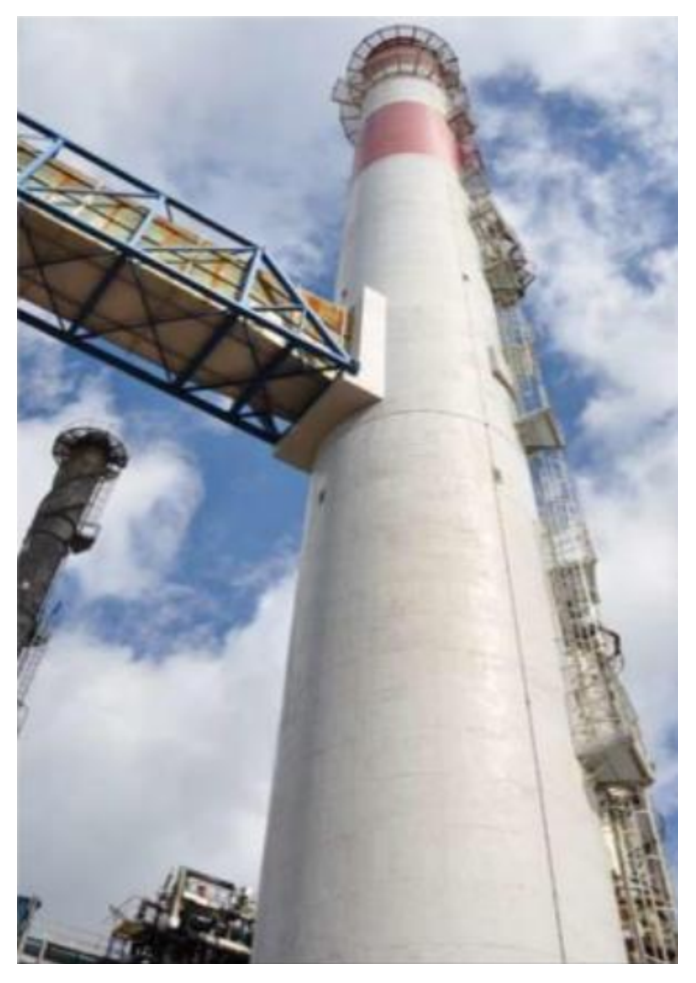
\includegraphics[height=40mm]{donges_chimney.eps}\label{sfig:donges_chimney}}
    \subfloat[]{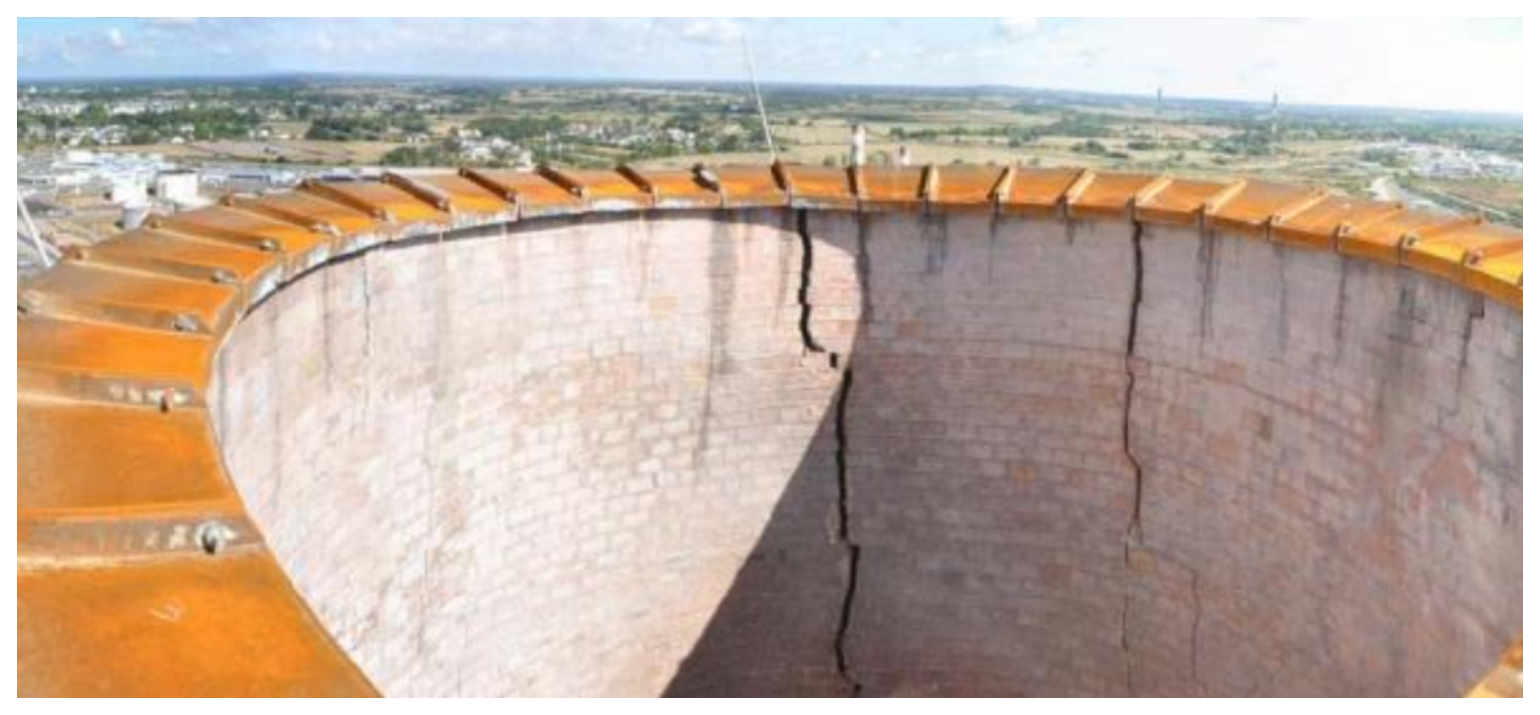
\includegraphics[height=40mm]{donges_chimney_fractures.eps}\label{sfig:donges_chimney_fractures}}
    \caption{(a) Image of the Donges gas chimney. (b) Image of the fractures within the inner masonry coating of the gas chimney. Courtesy of Delta International, 2010}
    \label{fig:donges_chimney}
\end{figure}
The structure essentially composes of an inner masonry hollow cylinder and an external reinforced concrete coating. Several coatings have been added to the structure but will not be considered at all in the study, for the sake of simplicity. The masonry layer thickness $e_{m}(z)$ depends on the elevation $z$: $e_m(z)=e_{m1}$ for $0\le z \le H_m$=6.57 m and $e_m(z)=e_{m2}$ for $H_m\le z\le H$. In particular, $e_{m1}$=20 cm and $e_{m2}$=10 cm. The concrete thickness $e_c(z)$ decreases linearly along the altitude, from the base to the height $H_c$=33.5 m and then it remains constant from $z=H_c$ to $z=H$, i.e.  $e_c(z)=\max($35 cm-0.004$\cdot z$,20 cm$)$ . The foundation slab is circular, with a diameter of $D_f$=11 m and a thickness of $e_f$=2 m. The foundation slab is anchored to the ground via concrete piles. \\ 

\begin{figure}
    \centering
    \includegraphics[height=120mm]{Figures/Chimney_Section_crop.pdf}
    \caption{Technical drawing of the chimney with cross sections.}    
    \label{fig:tech_Chimney}
\end{figure}

According to an inspection report, drafted in 2010 following the explosion of an apparatus close to the chimney - that could have damaged it - several internal cracks in the masonry layer were detected, although they seemingly left the external concrete coating unaffected. The internal cracks are vertical, as shown in \Cref{sfig:donges_chimney_fractures}. The
several cracks in the brick lining pose a serious collapse potential. Moreover, despite the rather good conditions, the visual inspection reported a specific area (less than 1 m$^\text{2}$) where the reinforced concrete seemingly suffered of a chemical attack. The report suggested a deeper investigation into this area to identify if the reinforcement has been weakened. \\ Following
this inspection report, TotalEnergies retrofitted the chimney and commissioned SOCOTEC Monitoring the structural health monitoring of the chimney, to suggest a life expectancy to plan the rebuilding.


\subsection{Plan of the paper}
\label{subsec:plan_of_the_paper}
\textcolor{red}{To be drafted after the paper is done.}

\section{Data}
\label{sec:Data}
Following the incident, SOCOTEC Monitoring installed two one-dimensional (1-D) accelerometers at the very top of the chimney to monitor its dynamic structural behaviour. The accelerometers measure radial and tangential accelerations respectively, namely $\ddot{u}_r(t)$ and $\ddot{u}_\theta(t)$. The chimney was firstly instrumented in 2016 and monitored until 2017, for a few months. After a break of a few years, the two devices were reactivated in early 2020, before a new interruption. The instrumentation is now active since January 2021. The digital signals were recorded - twice a day, once at midnight and once at midday - by a data acquisition system installed at the base of the chimney, thanks to a 3G antenna. Each acquisition consists of time-histories of 15 min length, sampled at 100 Hz. This corresponds to a set of discrete acceleration time-histories of $M$ = 90000 sampling points, with a time-step $\Delta t$ = 0.01 s. \textcolor{red}{Filippo: add examples of recordings}.
\textcolor{red}{Raphaël: can we publish the database open source? - Yes but without mentioning Total in the article}


In the present study, for each $i^\text{th}$ acquisition, the acceleration time-histories (i.e. the data snapshots of that specific $i^\text{th}$ acquisition) are arranged into two $1\times M$ vectors $\St[r][(i)]$ (radial snapshot) and $\St[\theta][(i)]$ (tangential snapshot), that read:
$$\St[r][(i)]=\bmat[\ddot{u}^{(i)}_r(0),\ddot{u}^{(i)}_r(\Delta t),\ldots ,\ddot{u}^{(i)}_r((M-1)\Delta t)][cccc] \quad \St[\theta][(i)]=\bmat[\ddot{u}^{(i)}_\theta(0),\ddot{u}^{(i)}_\theta(\Delta t),\ldots ,\ddot{u}^{(i)}_\theta((M-1)\Delta t)][cccc]$$
For the sake of simplicity, each $i^{\text{th}}$ acquisition, starting at absolute time $t_i$, is referenced in time starting at local time $\tau^{(i)}=0$, where $\tau^{(i)}=t-t_i$.\\ For this purpose, the following \textit{time extraction operator} is also defined:
\begin{equation}
    \label{eq:time_extracion}
    \mathcal{E}_j^k(\St[][(i)]) = \bmat[\ddot{u}^{(i)}(j\Delta t),\ddot{u}^{(i)}((j+1)\Delta t),\ldots ,\ddot{u}^{(i)}_\theta((k-1)\Delta t)][cccc]
\end{equation}
The \textit{time extraction operator} indistinctly applies to both $\St[r][(i)]$ and $\St[\theta][(i)]$ (which is why it is applied to a generic snapshot $\St[][(i)]$ in \Cref{eq:time_extracion}. It extracts from the $i^\text{th}$ acquisition snapshot the subset of contiguous discrete values acquired between the $j^\text{th}$ and $k^\text{th}$ time-steps (local acquisition time $\tau^{(i)}$).\\

\textcolor{red}{Attention: we talk of non-linear modelling, but the model used for calibration and for sensitivity analysis is linear.}

\section{Methods}
\label{sec:methods}

\textcolor{red}{We need a graph explaining how the different tools (parametric DMD + sensitivity analysis + numerical model)}

\subsection{Elementary effects method}
\textcolor{red}{check possible repetition with the content of the introduction section}

Determining and monitoring elastic properties is a widespread approach for detecting damage \cite{art:Pandey94}. Dynamic identification can be carried out by comparing numerical predictions with experimental data and by modifying material parameters on the basis of their discrepancy. In this work, material parameters are collected in a vector $\boldsymbol{\eta}\in \mathbb{R}^{N_\eta}$, and FE based numerical models are employed to predict structural frequencies $\boldsymbol{\lambda}_{\text{num}}=y(\boldsymbol{\eta})$. At the early stage of a monitoring process, structural frequencies $\boldsymbol{\lambda}_{\text{exp}}$ are employed to determine a reference configuration \cite{art:Kamariotis21}. The onset and propagation of damage is monitored with respect to this configuration \cite{thesis:PhD}.

It is not trivial to set how many and which parameters can be calibrated. With this goal, a sensitivity Analysis (SA) approach is adopted \cite{chp:Saltelli07_1}, levaing considerations on the observability and on the identifiability of the system \cite{art:Kalman63} for future work. Generally speaking, SA is used to quantify how the uncertainity of the model input affects the model output. Here, uncertainty is due to the dispersion of the mechanical properties of the construction materials, and to the possible onset and propagation of damage. A priori, it is just possible to define a suitable interval to which the material properties, namely the Young modulus of concrete and masonry, belong to. A posteriori, it is then possible to refine this estimate by comparing numerical outputs and measurements. However, some inputs affect only a little the model output. As it would be impossible to provide a menaningful estimate of these inputs, SA is exploited to exclude these parameters from the identification \cite{chp:Saltelli07_1}.

The elementary effects method \cite{art:Morris91} is here employed. It consists in computing two indices $\mu_i$ and $\sigma^2_i$ for each model input $\eta_i$, with $i=1,\ldots,N_{\eta}$: $\mu_i$ specifies if the effect of $\eta_i$ is linear and additive; $\sigma^2_i$ if the effect of $\eta_i$ is non--linear or involve in interactions with other inputs. The indices $\mu_i$ and $\sigma^2_i$ are good proxy for Sobol' indices \cite{art:Sobol01} but require smaller computational resources, a crucial aspect managing quite expensive FE codes. 
%If a greater number of degrees of freedom (dofs) were employed, a version of the elementary effect method based on more effective screening design would be recommendable \cite{art:Campolongo07}.

To compute $\mu_i$ and $\sigma^2_i$, a number of incremental ratios $EE_i$ termed Elementary Effects (EE) are computed for each $\mu_i$ as follows:
\begin{equation}
    EE_i = \frac{y(\eta_1,\ldots,\eta_i+\Delta,\ldots,\eta_{N_{\eta}})-y(\eta_1,\ldots,\eta_{N_{\eta}})}{\Delta},
\end{equation}
where: $\Delta$ is a value in $\lbrace 1/(p-1), \ldots, 1-1/(p-1) \rbrace$; $p$ is the number of levels in which the $N_{\eta}$--dimensional unit cube, describing the sample space of $\boldsymbol{\eta}$, is divided.

The sensitivity indices coincide with the basic statistics of the distribution to which $EE_i$ belong. This implies that:
\begin{subequations}
\begin{gather}
    \mu_i = \frac{1}{N_r}\sum^{N_r}_{n_r=1} EE^{n_r}_i \\
    \sigma^2_i = \frac{1}{N_r-1}\sum^{N_r}_{n_r=1} (EE^{n_r}_i - \mu )^2,
\end{gather}
\end{subequations}
where $N_r$ is the number of sampled $EE_i$ or, in other words, the number of trajectories. Adopting the sampling strategy proposed in \cite{art:Morris91}, the total number of samples of the input space is equal to $N_r(N_{\eta}+1)$.

\begin{figure}
    \centering
    \subfloat[]{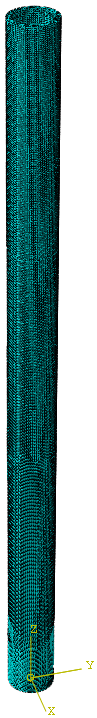
\includegraphics[height=60mm]{Figures/meshImageAbaqusModelChimney.PNG}\label{fig:meshChimney}}
    \subfloat[]{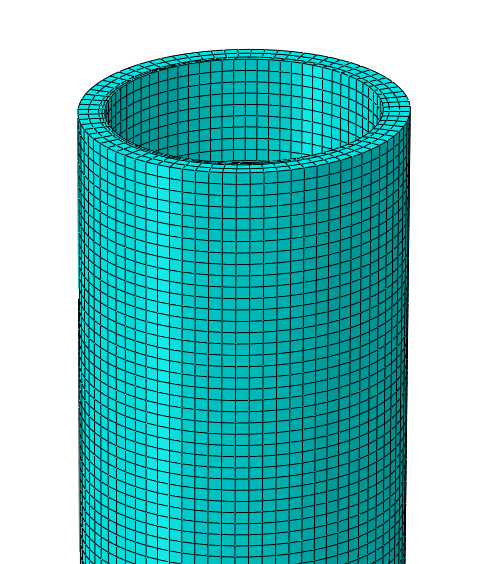
\includegraphics[height=40mm]{Figures/meshImageAbaqusModelChimney_detail.PNG}\label{fig:meshChimneyDetail}}
    \caption{Mesh employed by the finite element model of the chimney (on the right: detail).}    
    \label{fig:mesh_Chimney}
\end{figure}

\subsection{Dynamic system modelling}
\label{sec:dynSystemModelling}
In this study, the oscillating gas chimney is represented by the following non-linear dynamic system:
\begin{equation}
    \matd[\Vv]=\fv\pdp{\Vv(t)}
    \label{eq:nonlinear_dynamics}
\end{equation}
with $\Vv(t)\in \mathcal{M}$ (the so called \textit{phase space}) being the vector of particle velocities at some spatial locations $\xv[j]$, such as the node positions of a Finite Element mesh of the chimney or the sensors' locations. In general, the vector $\Vv(t)$ represents the set of degrees of freedom of the chimney digital twin.\\ Intuition led to consider the chimney as a non-linear dynamic system, given the past explosion reported at the Donges refinery and the presence of visible fractures in the inner masonry coating (see \Cref{sfig:donges_chimney_fractures}). Dynamic systems are usually discretized in time, at discrete time instances $t_k \in \R$ with time index $k\in {0} \cup \N$. In this sense, the time-marching integration scheme, applied to \Cref{eq:nonlinear_dynamics} reads~\cite{brunton_chaos_2017}:
\begin{equation}
    \Vv(t_{k+1})=\Fv(\Vv(t_{k}))=\Vv(t_{k})+\int_{t_k}^{t_{k+1}} \fv(\Vv(s)) ds
    \label{eq:nonlinear_dynamics_discrete}
\end{equation}
The non-linear functional $\Fv:\mathcal{M}\to\mathcal{M}$ defined in \Cref{eq:nonlinear_dynamics_discrete} is deterministic and defined over the probability space $(\mathcal{M},\Sigma_\mathcal{M},\mu_\mathcal{M})$. However, one can consider random dynamic systems (RDS), by explicitly including the so called \textit{process noise}~\cite{takeishi_subspace_2017}. In this case, the discrete RDS is described by:
\begin{equation}
    \Vv(t_{k+1})=\Fv[\xi](\Vv(t_{k}),\xiv[t])
    \label{eq:RDS}
\end{equation}
with $\xiv[t]$ being the random noise defined over a probability space $(\Xi,\Sigma_\Xi,\mu_\Xi)$.\\ For the sake of clarity, in \Cref{subsec:Modal_identification_from_raw_data_with_Multiresolution_DMD}, $\Vv(t)=\bmat[\dot u_r\\ \dot u_\theta][c]$. \textcolor{red}{Define $\Vv(t)$ in other sections}

\subsection{Modal identification with Fourier analysis}
\label{subsec:Modal_identification_Fourier}
\textcolor{red}{
- Application of Fast Fourier Transform algorithm
- Peak detection algorithm to infer 3 first modal frequencies (f0, f1, f2)
- Hampel filter to filter outliers}

\subsection{Modal identification from raw data with Multiresolution DMD}
\label{subsec:Modal_identification_from_raw_data_with_Multiresolution_DMD}
In order to identify the non-linear modal behaviour of the structure, the raw data acquisitions are analysed with the Dynamic Modal Decomposition (DMD)~\cite{Rowley_et_al_2009,Schmid_2010,Schmid_et_al_2011,Tu_et_al_2014}. The DMD is an equation-free method that exploits the data snapshots $\St$, recorded at different spatial locations on the dynamical system at stake, to extract low-dimensional spatio-temporal modes. In particular, the DMD assumes an underlying linear dynamic system with $\Fv(\Vv(t))=\Av.\Vv(t)$, where $\Vv(t)=\bmat[\dot u_r\\ \dot u_\theta][c]$. This would imply that each time snapshot belongs to a Krylov subspace, i.e., for the present study it holds that $\mathcal{E}_0^{M-2}(\St[][(i)])=\psp{\ddot{u}(0),A\ddot{u}(0),\ldots,A^{M-2}\ddot{u}(0)}$ and $\mathcal{E}_1^{M-1}(\St[][(i)])=A\mathcal{E}_0^{M-2}(\St[][(i)])$. The DMD runs a least-squares regression over the data snapshots, so to find the best-fitting $A=\underset{A\in \R}{\arg\min}\norm{\mathcal{E}_1^{M-1}(\St[][(i)])-A\mathcal{E}_0^{M-2}(\St[][(i)])}$ and compute its eigenmodes~\cite{kutz_multiresolution_2016}. In order to avoid the well numerical degeneracy of the Krylov base for large $M$, the DMD considers a rank-reduced basis obtain via Proper Orthogonal Decomposition (POD) of $\Av$, i.e. it firstly computes the Singular Value Decomposition (SVD) of $\mathcal{E}_0^{M-2}(\St[][(i)])$, namely the $r$ right and left singular vectors $\Vt[r]\in\mathbb{C}^{r\times M}$ and $\Ut[r]\in\mathbb{C}^{1\times r}$ corresponding to the largest $r$ singular values ($r=1$ in this case) according to the following expression:
\begin{equation}
    \mathcal{E}_0^{M-2}(\St[][(i)])=\Ut[r]\Sigmat\Vt[r][*]
    \label{eq:svd}
\end{equation}
with $\Sigmat=\text{diag}(\tilde{\sigma}_i^2)$ represents the $r\times r$ diagonal matrix of singular values. Thereafter, the linear operator $\Av$ is rewritten as $\Av=\mathcal{E}_1^{M-1}(\St[][(i)])\Vt[r]\Sigmat[][-1]\Ut[r][*]$ and approximated by its $r\times r$ projection onto the POD modes $\tAv=\Ut[r][*]\Av\Ut[r]$. Once computed the right eigenvectors $\wv[k]$ of $\tAv$, associated to the eigenvalues $\lambda_k$, the low-rank approximated eigen-decomposition of $\Av$ is obtained as $\Psiv=\sum_{k}\psiv[k]\otimes\tens{\bar \psi}{k}{}=\sum_{k=1}^r\pdp{\mathcal{E}_0^{M-2}(\St[][(i)])\Vv[r]\Sigmat[][-1]\wv[k]}\otimes\tens{\bar \wv}{k}{}$. This eigen-decomposition allows to approximate the future prediction at each spatail coordinate within the snapshot $\xv[j]$ and therefore to predict the whole time-history and any future time step, according to the following expression:
\begin{equation}
    \vct{\tilde V}{}{}\Big\vert_{\xv[j]}(t)=\sum_{k=1}^r b_k(0) \cdot \phiv[k](\xv[j])\cdot e^{\frac{\log \lambda_k}{\Delta t}t}=\Psiv(\xv[j])\text{diag}\pdp{e^{\frac{\log \lambda_k}{\Delta t}t}}\bv
    \label{eq:DMD_approximation}
\end{equation}
with $\bv$ being the vector of initial conditions, i.e., $\bv=\Psiv[][\dag]\mathcal{E}_0^{0}(\St[][(i)])$, with $\Psiv[][\dag]$ indicating the Moore–Penrose pseudoinverse~\cite{Tu_et_al_2014}. In this section, the Multiresolution DMD (mrDMD) proposed by~\cite{kutz_multiresolution_2016} is adopted, which consists into iteratively applying the standard DMD to sub-snapshots obtained by successive time-splitting of the original. In practice, at each decomposition level $\ell$, the DMD is applied to each sub-snapshot (of length $T_h$) and the slowest 
$m^{(\ell)}$ modes are retained for the final modal sum, corresponding to the resolution level $\ell$. Thereafter, those $m^{(\ell)}$ modes are removed and the sum obtained by DMD at resolution level $\ell$ and the snapshot is time-split into two parts of length $T_{h+1}=\frac{T_{h}}{2}$ to start the next iteration.Compared to the traditional DMD algorithm, the mrDMD variant yields the following approximation:
\begin{equation}
    \vct{\tilde V}{}{}\Big\vert_{\xv[j]}(t)=\sum_{\ell=1}^L\sum_{h=1}^{2^{\ell-1}}\sum_{k=1}^{m^{(\ell)}} \chi^{(\ell)}_{[t_h,t_{h+1}]}(t)\cdot b_k^{(\ell,h)}(0) \cdot \phiv[k][(\ell,h)](\xv[j])\cdot e^{\frac{\log \lambda_k^{(\ell,h)}}{\Delta t}t}
    \label{eq:DMD_approximation}
\end{equation}
with $\chi^{(\ell)}_{[t_h,t_{h+1}]}(t)$ being the indicator function over the time interval $\psp{t_h,t_{h+1}}$ of duration $T_h$, corresponding to each of the $2^\ell$ sub-snapshot time-ranges. For the sake of simplicity, eigenmodes with wavelength shorter than the time window $T_h$ are retained. 
\subsection{Modal identification from raw data with subspace DMD}
\label{subsec:Modal_identification_from_raw_data_with_subspace_DMD}


It has been widely demonstrated (see~\cite{Rowley_et_al_2009,Schmid_2010,Mezic_2013,kutz_multiresolution_2016}) that the DMD method approximates the modes of the so-called \textit{Koopman operator}~\cite{Koopman_1931}. The Koopman operator $\mathcal{K}$ is an attractive tool to represent non-linear dynamic systems without linearization. As a matter of fact, $\mathcal{K}$ is an infinite-dimensional linear operator that applies to the space of possible observation functions $\gv:\mathcal{M}\to\mathbb{C}$ (of any quantity of interest of the system, in this case the acceleration time-histories $\ddot{u}_r$ and $\ddot{u}_\theta$, with $\gv\in\mathcal{G}\subset L^{2}(\mathcal{M},\mu_\mathcal{M})$, namely:
\begin{equation}
    \mathcal{K}\gv(\Vv) \overset{\Delta}{=} \gv\circ \Fv(\Vv)
    \label{eq:Koopman_operator}
\end{equation}
\Cref{eq:Koopman_operator} implies that $\mathcal{K}\gv(\Vv(t_k)) = \gv\circ \Fv(\Vv(t_k))=\gv(\Vv(t_{k+1}))$. Moreover, $\mathcal{K}(\alpha\cdot \gv[\alpha]+\beta \cdot \gv[\beta])=\alpha\cdot\mathcal{K} \gv[\alpha]+\beta\cdot\mathcal{K}\gv[\beta]$. The Koopman operator trades the finite-dimensional nature of the non-linear dynamic problem with a linear yet inifinite-dimensional representation, on the space of all the measurement functions $\mathcal{G}$~\cite{brunton_chaos_2017}. In practice, the Koopman operator becomes attractive when a finite-dimensional approximation can be obtained, i.e. when a convenient finite-dimensional subspace $G\subset\mathcal{G}$ invariant to $\mathcal{K}$ is obtained. In other words, $G$ must be chosen so that $\mathcal{K}g\in G, \forall g\in \mathcal{G}$~\cite{takeishi_subspace_2017}. In practice, this task can be harder than to obtain the solution of the original system~\cite{brunton_chaos_2017}, but in such a way, the restriction of $\mathcal{K}$ to $G$, namely $K$ is finite-dimensional too. As a matter of fact, if ones suppose to have a finite set of observation functions $\Gt=\psp{\gv[1], \ldots, \gv[n]}$ with $n<\infty$, then the representation of $K$ over $\gv$ is expressed as $K\Gt$. With such finite-dimensional approximation of the Koopman operator, $G$ is spanned by the right eigenvectors $\uv[i]$ of $K$ and $\gv\in G$ can be written as a linear combination of the $n$ eigenvectors (\textit{Koopman modes} of the map $\Fv$) multiplied by the corresponding $K$'s eigenfunctions $\varphi_i(\Vv)$ (\textit{Koopman eigenfunctions}), i.e.  $\gv=\sum_i \varphi_i(\Vv)\cdot \uv[i]$~\cite{Rowley_et_al_2009}. The DMD approximates the Koopman modes and it can be therefore applied to nonlinear systems. 

\section{Results}
\label{sec:results}

\subsection{Sensitivity analysis outcomes}
\label{sec:results_SA}
\begin{figure}
    \centering
    \subfloat[]{\includegraphics[height=60mm]{Figures/DisegnoPartizione_con_sezione_crop2.pdf}\label{fig:disegnoPartizione}}
    \subfloat[]{\includegraphics[height=40mm]{Figures/meanStandardEE_crop.pdf}\label{fig:SAoutcomes}}
    \caption{Chimney material subdivision.}    
    \label{fig:disegnoPartizione_SAoutcomes}
\end{figure}



 
% Please note that the first paragraph of a section or subsection is
% not indented. The first paragraph that follows a table, figure,
% equation etc. does not need an indent, either.

% Subsequent paragraphs, however, are indented.

% \subsubsection{Sample Heading (Third Level)} Only two levels of
% headings should be numbered. Lower level headings remain unnumbered;
% they are formatted as run-in headings.

% \paragraph{Sample Heading (Fourth Level)}
% The contribution should contain no more than four levels of
% headings. Table~\ref{tab1} gives a summary of all heading levels.

% \begin{table}
% \caption{Table captions should be placed above the
% tables.}\label{tab1}
% \begin{tabular}{|l|l|l|}
% \hline
% Heading level &  Example & Font size and style\\
% \hline
% Title (centered) &  {\Large\bfseries Lecture Notes} & 14 point, bold\\
% 1st-level heading &  {\large\bfseries 1 Introduction} & 12 point, bold\\
% 2nd-level heading & {\bfseries 2.1 Printing Area} & 10 point, bold\\
% 3rd-level heading & {\bfseries Run-in Heading in Bold.} Text follows & 10 point, bold\\
% 4th-level heading & {\itshape Lowest Level Heading.} Text follows & 10 point, italic\\
% \hline
% \end{tabular}
% \end{table}


% \noindent Displayed equations are centered and set on a separate
% line.
% \begin{equation}
% x + y = z
% \end{equation}
% Please try to avoid rasterized images for line-art diagrams and
% schemas. Whenever possible, use vector graphics instead (see
% Fig.~\ref{fig1}).

% \begin{figure}
% 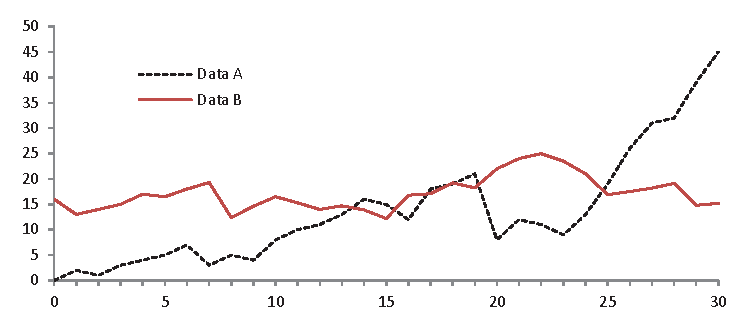
\includegraphics[width=\textwidth]{fig1.eps}
% \caption{A figure caption is always placed below the illustration.
% Please note that short captions are centered, while long ones are
% justified by the macro package automatically.} \label{fig1}
% \end{figure}

% \begin{theorem}
% This is a sample theorem. The run-in heading is set in bold, while
% the following text appears in italics. Definitions, lemmas,
% propositions, and corollaries are styled the same way.
% \end{theorem}
% %
% % the environments 'definition', 'lemma', 'proposition', 'corollary',
% % 'remark', and 'example' are defined in the LLNCS documentclass as well.
% %
% \begin{proof}
% Proofs, examples, and remarks have the initial word in italics,
% while the following text appears in normal font.
% \end{proof}
% For citations of references, we prefer the use of square brackets
% and consecutive numbers. Citations using labels or the author/year
% convention are also acceptable. The following bibliography provides
% a sample reference list with entries for journal
% articles~\cite{ref_article1}, an LNCS chapter~\cite{ref_lncs1}, a
% book~\cite{ref_book1}, proceedings without editors~\cite{ref_proc1},
% and a homepage~\cite{ref_url1}. Multiple citations are grouped
% \cite{ref_article1,ref_lncs1,ref_book1},
% \cite{ref_article1,ref_book1,ref_proc1,ref_url1}.

\section*{Acknowledgments}
\label{sec:acknowledgments}
This paper was sponsored by SOCOTEC Monitoring, in the framework of collaboration with CentraleSupélec. SOCOTEC Monitoring sponsored the team of co-authors C. Kfoury, F. Pinard and T. Zerr, in the context of their undergraduate engineering project at CentraleSupélec, called \textit{Jean Muller} project, proposed by the third-year \textit{Sciences et Ingénieries de la Constructions} track at CentraleSupélec.
%
% ---- Bibliography ----
%
% BibTeX users should specify bibliography style 'splncs04'.
% References will then be sorted and formatted in the correct style.
%
\bibliographystyle{splncs04}
\bibliography{mybibliography}

\end{document}